\documentclass[a4page]{article}
\usepackage[T1]{fontenc}
\usepackage[utf8]{inputenc}
\usepackage[italian]{babel}
\usepackage{index}
\usepackage{booktabs}
\usepackage{longtable}
\usepackage{array}
\usepackage{graphicx}
\usepackage{ulem}
\usepackage[table,xcdraw]{xcolor}
\usepackage[T1]{fontenc}
\usepackage{hyperref}
\usepackage{xcolor,listings}
\usepackage[vmargin=2cm]{geometry}
\usepackage{color}
\usepackage{lscape}
\usepackage{imakeidx}
\usepackage{fancyvrb}
\definecolor{dkgreen}{rgb}{0,0.6,0}
\definecolor{gray}{rgb}{0.5,0.5,0.5}
\definecolor{mauve}{rgb}{0.58,0,0.82}
\usepackage{titlesec, blindtext, color}
\definecolor{gray75}{gray}{0.75}
\usepackage{textcomp}
    \usepackage{color}

    \definecolor{codegreen}{rgb}{0,0.6,0}
    \definecolor{codegray}{rgb}{0.5,0.5,0.5}
    \definecolor{codepurple}{HTML}{C42043}
    \definecolor{backcolour}{HTML}{F2F2F2}
    \definecolor{bookColor}{cmyk}{0,0,0,0.90}  
    \color{bookColor}

    \lstset{upquote=true}

    \lstdefinestyle{mystyle}{
        backgroundcolor=\color{backcolour},   
        commentstyle=\color{codegreen},
        keywordstyle=\color{codepurple},
        numberstyle=\footnotesize\color{codegray},
        stringstyle=\color{codepurple},
        basicstyle=\footnotesize,
        breakatwhitespace=false,         
        breaklines=true,                 
        captionpos=b,                    
        keepspaces=true,                 
        numbers=left,                    
        numbersep=-10pt,                  
        showspaces=false,                
        showstringspaces=false,
        showtabs=false,      
    }
    \lstset{style=mystyle} 
\newcommand{\hsp}{\hspace{20pt}}
\titleformat{\chapter}[hang]{\Huge\bfseries}{\thechapter\hsp\textcolor{gray75}{|}\hsp}{0pt}{\Huge\bfseries}

\begin{document}
% inizio pagina@@@@
\clearpage
% command to provide stretchy vertical space in proportion
\newcommand\nbvspace[1][3]{\vspace*{\stretch{#1}}}
% allow some slack to avoid under/overfull boxes
\newcommand\nbstretchyspace{\spaceskip0.5em plus 0.25em minus 0.25em}
\begin{titlepage}
\begin{center}
\tt
\nbvspace[0.03]
\begin{tabular}[c]{@{}c@{}}\vspace{0.1cm}\textbf{\LARGE{UNIVERSITA' DEGLI STUDI DI NAPOLI FEDERICO II}}\\\vspace{0.1cm}\Large{SCUOLA POLITECNICA E DELLE SCIENZE DI BASE}\\\large{DIPARTIMENTO DI INGEGNERIA ELETTRICA E TECNOLOGIE DELL'INFORMAZIONE}\end{tabular}


\includegraphics[width=4cm]{LOGO}
\nbvspace[0.1]
\begin{tabular}[c]{@{}c@{}}\vspace{0.1cm}\Large{CORSO DI LAUREA IN INFORMATICA}\\\vspace{0.1cm}\Large{INSEGNAMENTI DI BASI DI DATI E PROGRAMMAZIONE AD OGGETTI}\\\Large{ANNO ACCADEMICO 2022/2023}\end{tabular}
\rm
\begin{tabular}[c]{@{}c@{}}\huge{\textbf{Progettazione e sviluppo di una base di dati}}\\\huge{\textbf{relazionale per la descrizione e la}}\\\huge{\textbf{memorizzazione di conferenze scientifiche}}\end{tabular}
\end{center}
\begin{longtable}[c]{llr}
\textit{Autori:}                                                                                                                   &  & \textit{Docenti:}                                                                        \\
\endhead
%
\begin{tabular}[c]{@{}l@{}}ALESSANDRO GRIECO\\      Matricola N86/4241\\      alessandro.grieco2@studenti.unina.it\end{tabular}    &  & \begin{tabular}[c]{@{}r@{}}Prof. Mara SANGIOVANNI\end{tabular} \\
\begin{tabular}[c]{@{}l@{}}GIANFRANCO DUMINUCO\\      Matricola N86/4061\\      gianfranco.duminuco@studenti.unina.it\end{tabular} &  & \multicolumn{1}{l}{}                                                                    
\end{longtable}                  
\end{titlepage}
\tableofcontents
\newpage
\vspace{10cm}
\section{PREFAZIONE}
Si provvederà alla progettazione e sviluppo di una base di dati dedicata alla gestione di conferenze. La base di dati permetterà di effettuare modifiche a conferenze già esistenti, di inserire conferenze future e visualizzare specifici dati riguardanti tutto ciò di cui una conferenza è composta.
\subsection{Conferenza, sede, programma, locazione e sessione}
Questo insieme di entità sono lo scheletro di una conferenza, permettono di identificare le informazioni sulla data/orario/luogo della conferenza:
\begin{itemize}
\item \textbf{conferenza} : Fornisce dati generali sulla trattazione e organizzazione temporale della conferenza;
\item \textbf{programma e sessione} : Consentono di conoscere gli orari e argomenti delle varie sedute della conferenza;
\item \textbf{sede e locazione} : Definiscono il luogo fisico in cui si terranno le varie sessioni di una conferenza.
\end{itemize}
\subsection{Evento sociale e intervallo}
Consentono ad un partecipante e/o ad un organizzatore di identificare i momenti di pausa ed i momenti di eccezione di una conferenza
\subsection{Organizzatore locale, organizzatore scientifico, partecipante, intervento ed ente}
Questo gruppo di entità costituisce la base delle varie sessioni di una conferenza. Compongono la popolazione di una conferenza, come questa partecipa alle varie sessioni e come questa si muove all'interno di una conferenza.
\begin{itemize}
\item \textbf{ente} : Specifica l'ente di appartenenza di ciascun elemento appartenente alla popolazione di una conferenza;
\item \textbf{Organizzatore locale e scientifico} : Definisce le persone fisiche che organizzano una conferenza;
\item \textbf{partecipante e intervento} : Il partecipante è lo spettatore fisico di una sessione, il quale può intervenire o meno all'interno di essa.
\end{itemize}
\subsection{Sponsor e pubblicità}
Determinano l'insieme delle aziende le quali contribuiscono (anche economicamente) alla realizzazione di una conferenza.
\newpage
\section{PROGETTAZIONE CONCETTUALE}
In seguito sono riportati il diagramma ER e il rispettivo class diagram:
\subsection{ER}
\vspace{2cm}
\begin{figure}[h!]
\centering
\includegraphics[width=16cm]{ER}
\end{figure}
\newpage
\subsection{CLASS DIAGRAM}
\vspace{2cm}
\begin{figure}[h!]
\centering
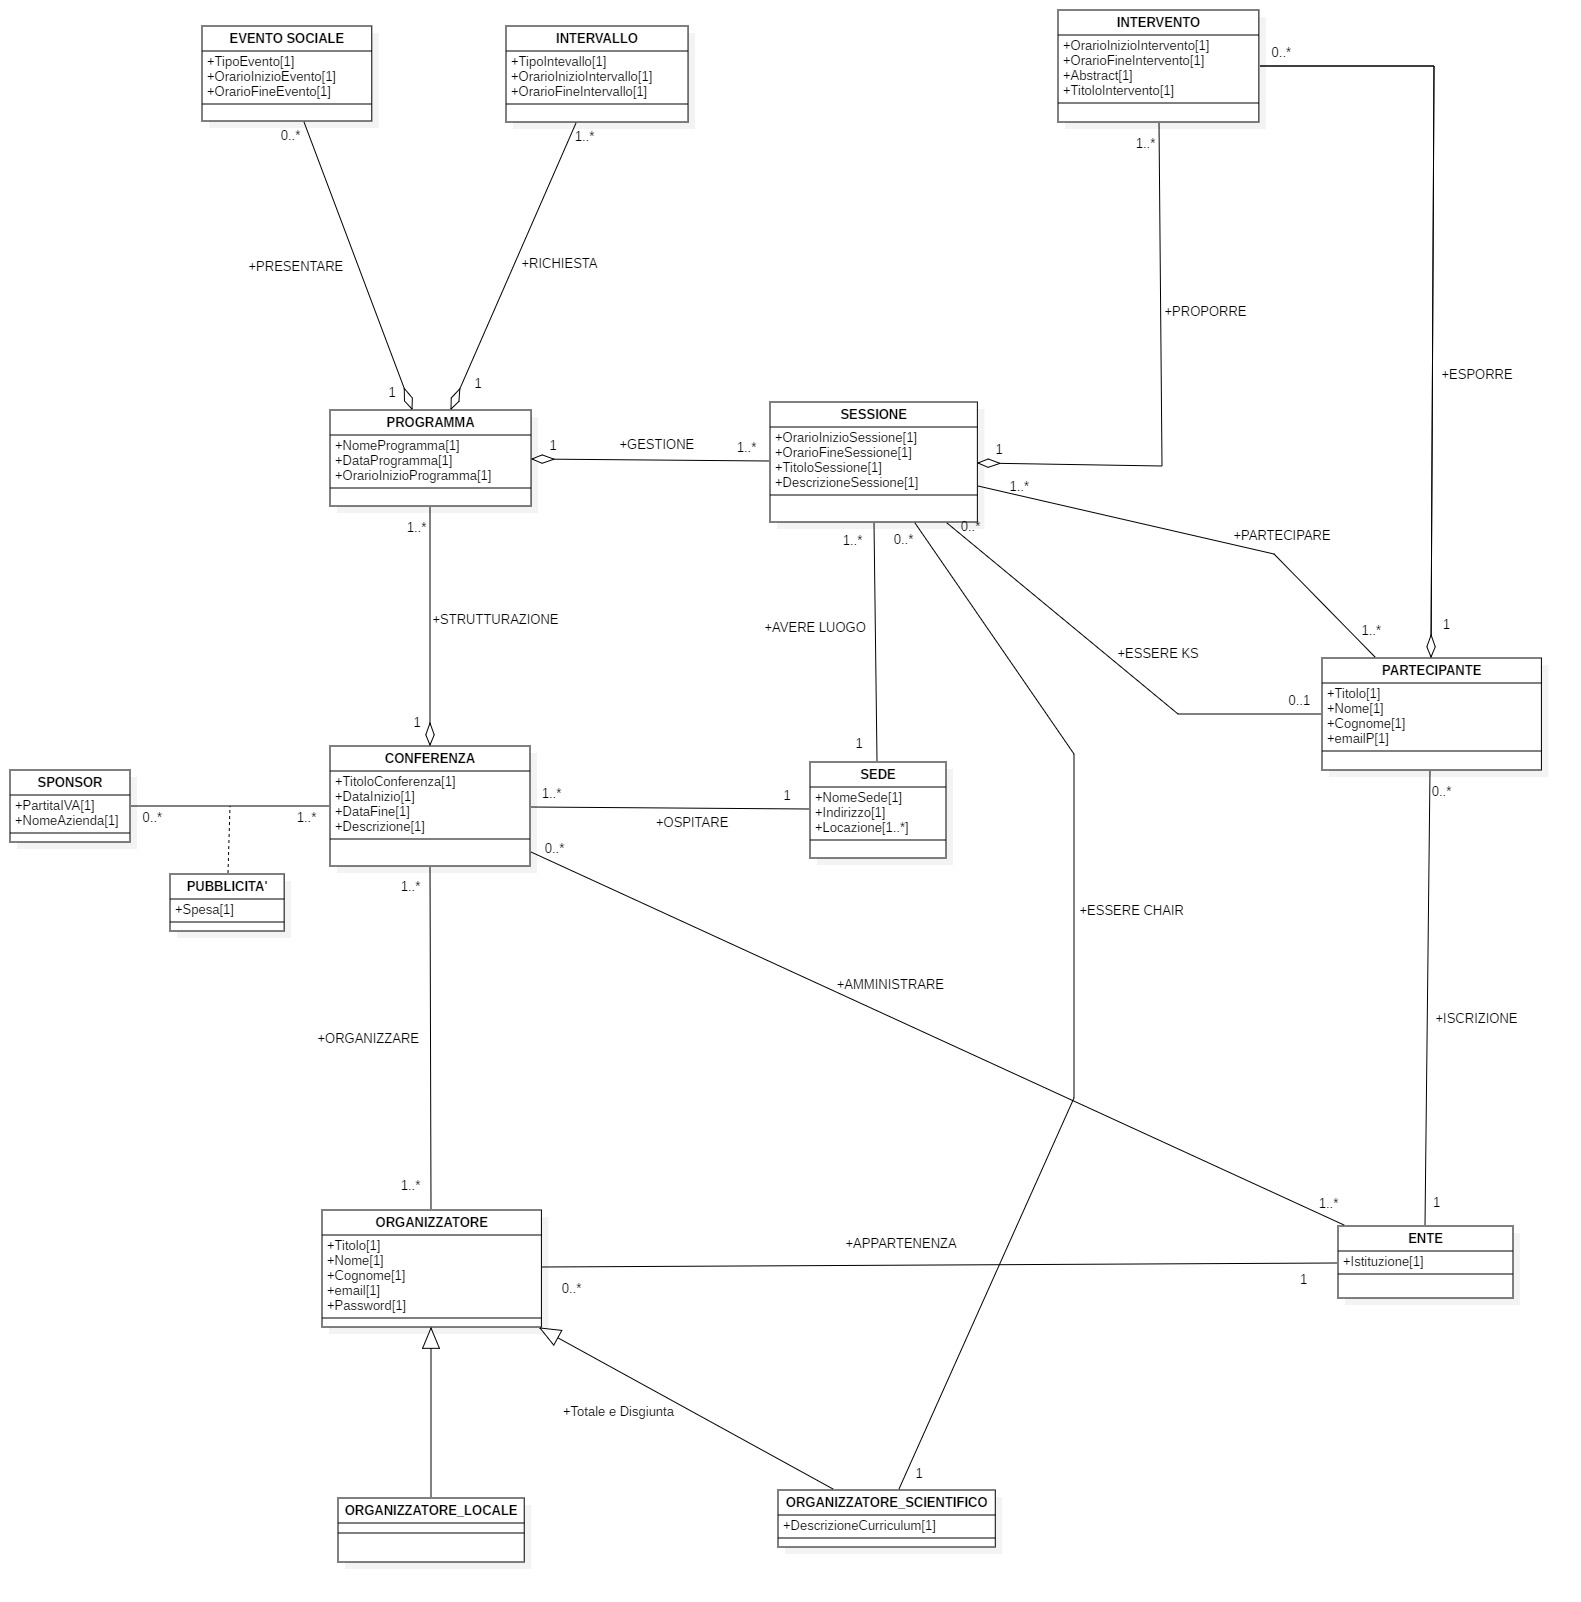
\includegraphics[width=17cm]{CSNR}
\label{mycsnr}
\end{figure}
\newpage
\vspace{2cm}
\subsection{Ristruttuazione del class diagram}
Per motivi di implementazione fisica è necessario ristrutturare il class diagram sopracitato \ref{mycsnr}, tenendo conto dei seguenti punti:
\paragraph{\textit{Eliminazione attributi multivalore}}
L'unico attributo multivalore presente nel diagramma risulta essere l'attributo locazione nell'entità sede, quindi è necessario rendere quest'ultimo un entità a sé stante. 
% aggiungere foto dettagliata su locazione e come diventa%
\paragraph{\textit{Eliminazione attributi strutturati}}
L'unico attributo strutturato risulta essere l'attributo indirizzo all'interno dell'entità sede, il quale può essere ristrutturato componendolo nei suoi sotto-attributi (NomeVia, NumeroCivico, Città)
% aggiungere foto dettagliata su indirizzo e come diventa%
\paragraph{\textit{Scelta degli identificatori primari}}
Per le entità sessione, programma, conferenza, intervento, intervallo, evento sociale sono state introdotte delle chiavi surrogate (rispettivamente codsessione, codprogramma, codconferenza, codintervento, codintervallo, codevento).
Per le entità sponsor, partecipante, organizzatore locale, organizzatore scientifico, ente, locazione e sede sono stati identificate come chiavi attributi preesistenti (rispettivamente PartitaIva, emailP, emailL, emailS, NomeIstituzione, NomeLocazione, NomeSede).
\paragraph{\textit{Eliminazioni delle gerarchie}}
L'unica gerarchia identificata (totale e disgiunta) nel class diagram è quella tra organizzatore, organizzatore scientifico ed organizzatore locale. Poiché l'entità organizzatore scientifico è totale e disgiunta, è possibile andare ad accorpare gli attributi dell'entità padre all'interno delle entità figlie.
% aggiungere foto bla bla%
\paragraph{\textit{Analisi delle ridondanze}}
Nel class diagram non sono presenti ridondanze.
\newpage
\subsection{CLASS DIAGRAM RISTRUTTURATO}
\vspace{2cm}
\begin{figure}[h!]
\centering
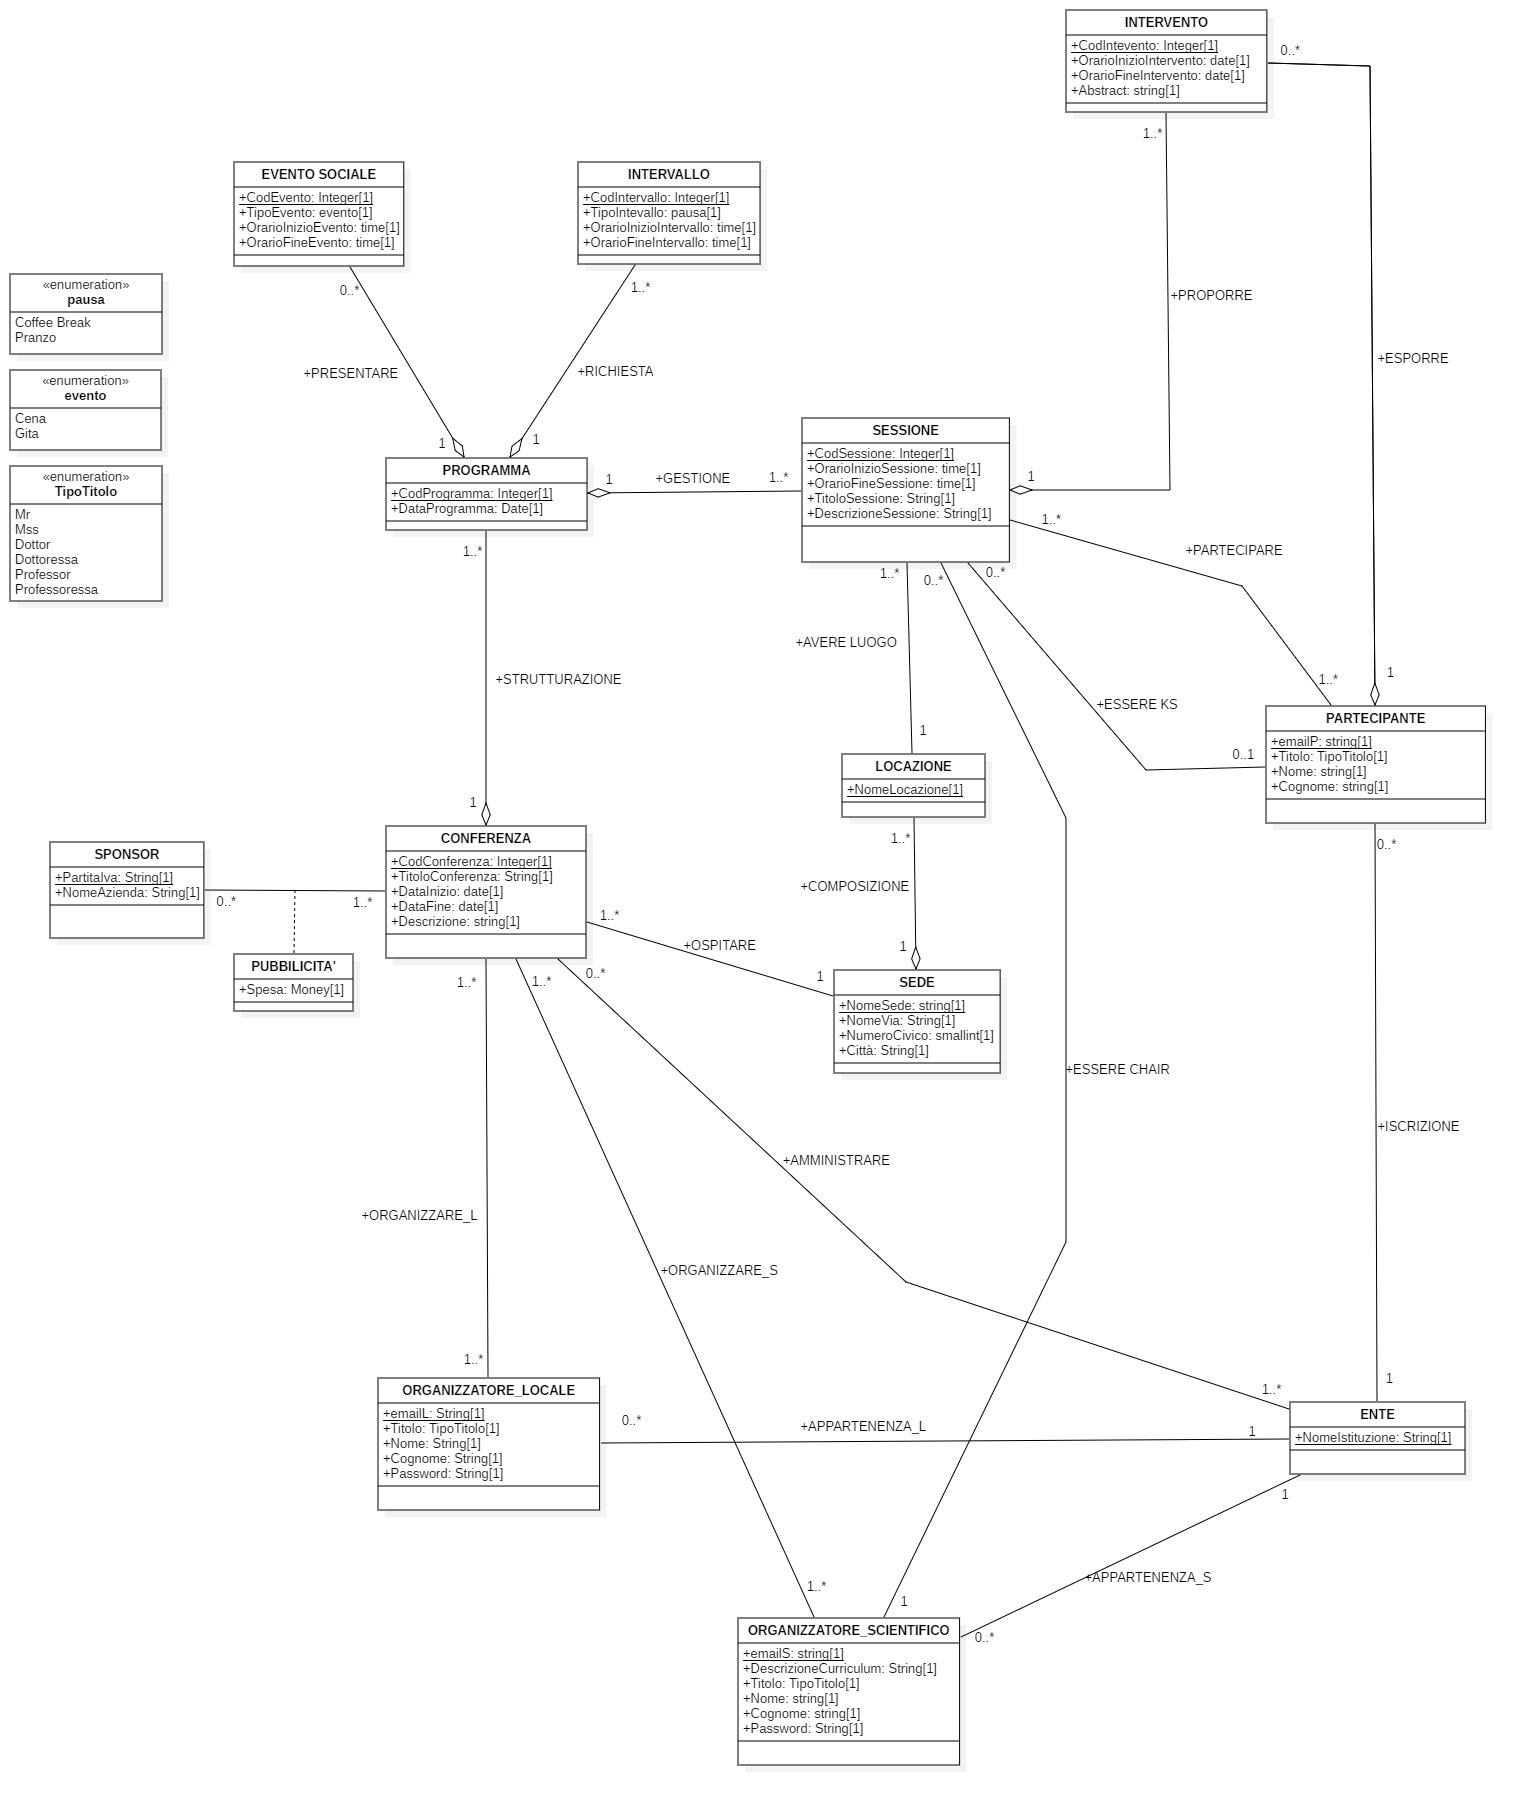
\includegraphics[width=16.5cm]{CSR}
\end{figure}
\newpage
\subsection{Dizionario classi}

\setlength{\LTleft}{-70pt}
\setlength\LTright{0pt}
\renewcommand\arraystretch{1.5}
\begin{longtable}{@{\extracolsep{\fill}}ccl}
\toprule
\multicolumn{1}{c}{\textbf{CLASSE}} & \multicolumn{1}{c}{\textbf{DESCRIZIONE}}                                                                                                                                                     & \textbf{ATTRIBUTI}                                                                                                                                                                                                                                                                                                                                                                                                                                                                                                                                                                                                                                                                                                                          \\ \bottomrule
\endhead
%
\textbf{CONFERENZA}                 & \begin{tabular}[c]{@{}c@{}}\vspace{-0.2cm}Riunione di rappresentanti di vari enti, \\ \vspace{-0.2cm}per uno scambio di vedute su problemi \\ \vspace{-0.2cm}di attualità o per risolvere una controversia \\ internazionale\end{tabular} & \begin{tabular}[c]{@{}l@{}}\vspace{-0.2cm}\textbf{CodConferenza} (integer): Chiave tecninca.\\ \vspace{-0.2cm}Identifica univocamente ciascuna istanza\\ di Conferenza.\\\vspace{-0.2cm}\textbf{DataInizio} (date) : Data in cui ha luogo la \\ Conferenza.\\ \vspace{-0.2cm}\textbf{DataFine} (data) : Data ove termina \\la Conferenza.\\ \vspace{-0.2cm}\textbf{Descrizione} (string) : Testo che illustra \\gli obiettivi della Conferenza.\\\vspace{-0.2cm}\textbf{TitoloConferenza} (string) : Nome che identifica \\la Conferenza.\end{tabular}                                                                                     \\ \hline
\textbf{SEDE} & \begin{tabular}[c]{@{}c@{}}Luogo fisico ove si tiene la conferenza\end{tabular} &\begin{tabular}[c]{@{}l@{}}\vspace{-0.2cm}\textbf{NomeSede} (string) : Nome identificativo \\\vspace{-0.2cm}della sede. Identifica univocamente le istanze\\ di Sede.\\\vspace{-0.2cm}\textbf{NomeVia} (string) : Nome nella strada in \\cui è presente la Sede.\\\vspace{-0.2cm}\textbf{NumeroCivico} (integer):Numero effettivo\\ della strada\\\vspace{-.2cm}\textbf{Città} (string): Comune dove è presente\\la Sede\end{tabular}
\\ \hline
\textbf{LOCAZIONE} & \begin{tabular}{@{}c@{}}\vspace{-0.2cm}Struttura interna alla sede \\ove si tiene la sessione \end{tabular} & \begin{tabular}{@{}l@{}}\vspace{-0.2cm}\textbf{NomeLocazione} (string) : Nome della\\locazione

\end{tabular} \\ \hline
\textbf{PROGRAMMA}                  & \begin{tabular}[c]{@{}c@{}}\vspace{-.2cm}Gestore della conferenza per migliorare\\ \vspace{-.2cm}la programmazione delle sedute\\ della conferenza\end{tabular}                                                          & \begin{tabular}[c]{@{}l@{}}\vspace{-.2cm}\textbf{CodProgramma} (integer) : Chiave tecnica.\\ \vspace{-.2cm} Identifica univocamente ciascuna istanza\\ di Programma.\\ \vspace{-.2cm}\textbf{DataProgramma} (date) : Data in cui è programmata \\una giornata della conferenza\end{tabular}                                                                                                                                                                                                                                                                                                                                                                                                                                                                                                                                                                                                                                                                   \\ \hline
\textbf{SESSIONE}                   & \begin{tabular}[c]{@{}c@{}}\vspace{-.2cm}Frammento di una conferenza avvenuta\\ in una data in un certo orario\end{tabular}                                                                                & \begin{tabular}[c]{@{}l@{}}\vspace{-.2cm}\textbf{CodSessione} (integer) : Chiave tecnica.\\\vspace{-.2cm} Identifica univocamente le istanze\\ di Sessione.\\\vspace{-.2cm}\textbf{OrarioInizioSessione} (time) : Orario inizio\\ della Sessione \\\vspace{-.2cm}\textbf{OrarioFineSessione} (time) : Orario fine della\\ Sessione.\\\vspace{-.2cm}\textbf{TitoloSessione} (string) : Denominazione\\ identificatrice della Sessione\\\vspace{-.2cm}\textbf{DescrizioneSessione} (string) : Testo illustrativo\\ degli obiettivi e discussione della Sessione.\end{tabular} \\ \hline
\textbf{PARTECIPANTE}               & \begin{tabular}[c]{@{}c@{}}\vspace{-0.2cm}Persona che partecipa\\ \vspace{-0.2cm}alla sessione in veste di\\ partecipante\end{tabular}                                                                                     & \begin{tabular}[c]{@{}l@{}}\vspace{-0.2cm}\textbf{emailP} (string): Indirizzo di posta elettrinica\\ \vspace{-0.2cm}del Partecipante. Identifica univocamente le\\ istanze di partecipante.\\ \vspace{-0.2cm}\textbf{Titolo} (TipoTitolo) : Carica accademica, professionale\\ o scientifica di rilievo (ex: dott./dott.ssa).\\ \textbf{Nome} (string) : Nome del partecipante.\\\textbf{Cognome} (string) : Cognome del partecipante.\end{tabular}                                                                                                                                                                                                                                                                                                                                                  \\ \hline
\textbf{INTERVENTO}                 & \begin{tabular}[c]{@{}c@{}}\vspace{-0.2cm}L'atto di prendere la parola\\  \vspace{-0.2cm}al fine di metter luce su\\ argomenti inerenti alla sessione\end{tabular}                                                         & \begin{tabular}[c]{@{}l@{}}\vspace{-0.2cm}\textbf{CodIntervento} (string) : Chiave tecnica.\\\vspace{-0.2cm} Identifica univocamente le istanze\\ di Intervento.\\ \vspace{-0.2cm}\textbf{OrarioInizioIntervento} (time) : Orario\\ che ha inizio l'Intervento.\\ \vspace{-0.2cm}\textbf{OrarioFineIntervento} (time) : Orario che\\ termine l'Intervento.\\ \vspace{-0.2cm}\textbf{Abstract } (string) : Breve testo il cui contenuto\\ descrive cosa verrà presentato dall'Intervento.\end{tabular}                                                                                                                                                                                                                                                                                                                                                                                                                        \\ \hline
\textbf{PUBBLICITA'}                 & \begin{tabular}[c]{@{}c@{}}\vspace{-0.2cm}Identifica il costo a spese dell'azienda\\ nel farsi pubblicità nella conferenza. \end{tabular}                                                         & \begin{tabular}[c]{@{}l@{}}\vspace{-0.2cm}\textbf{Spesa} (Money) : Costo pubblicitario per l'azienda\end{tabular}                                                                                                                                                                                                                                                                                                                                                                                                                        \\ \hline
\textbf{EVENTO SOCIALE}             & \begin{tabular}[c]{@{}c@{}}\vspace{-0.2cm}Celebrazione o commemorazione di\\ \vspace{-0.2cm}un particolare momento trascorso\\\vspace{-0.2cm} tra persone interessate alla tematica\\ della conferenza\end{tabular}                       & \begin{tabular}[c]{@{}l@{}}\vspace{-0.2cm}\textbf{CodEvento} (integer) :  Chiave tecnica.\\ \vspace{-0.2cm}Identifica univocamente le istanze di\\ Evento Sociale.\\ \vspace{-0.2cm}\textbf{TipoEvento} (evento) : Enumerazione\\ che specifica il tipo di evento (ex: Cena).\\ \vspace{-0.2cm}\textbf{OrarioInizioEvento} (time) : Orario d'inizio\\ dell'evento sociale.\\\vspace{-0.2cm}\textbf{OrarioFineEvento} (time) : Orario fine dell'evento \\ sociale.\end{tabular}                                                                                                                                                                                                                                                                                                                                                                                                                                              \\ \hline
\textbf{INTERVALLO}                 & \begin{tabular}[c]{@{}c@{}}\vspace{-0.2cm}Breve interruzione di un programma\\ \vspace{-0.2cm}o sessione che consente ai\\\vspace{-0.2cm} partecipanti di riposarsi prima della\\ sua continuazione\end{tabular}                          & \begin{tabular}[c]{@{}l@{}}\vspace{-0.2cm}\textbf{CodIntervallo} (integer) : Chiave tecnica.\\ \vspace{-0.2cm}Identifica univocamente le istanze\\ di Intervallo.\\ \vspace{-0.2cm}\textbf{TipoIntervallo} (pausa) : Enumazione che\\ specifica il tipo di intervallo (ex: coffee break)\\ \vspace{-0.2cm}\textbf{OrarioInizioIntervallo} (time) : Orario d'inizio \\ dell'Intervallo.\\ \vspace{-0.2cm}\textbf{OrarioFineIntervallo} (time) : Orario di fine\\ Intervallo\end{tabular}                                                                                                                                                                                                                                                                                                                                                                                                                                     \\ \hline
\textbf{\begin{tabular}[c]{@{}c@{}}ORGANIZZATORE\\ SCIENTIFICO\end{tabular}} & \begin{tabular}[c]{@{}c@{}}\vspace{-0.2cm}Responsabile della gestione\\\vspace{-0.2cm} su tematiche scientifiche e \\\vspace{-0.2cm} saccente su uno dei campi \\ che afferiscono alla conferenza\end{tabular}                            & \begin{tabular}[c]{@{}l@{}}\vspace{-0.2cm}\textbf{emailS} (string) : Indirizzo di posta elettronica.\\ \vspace{-0.2cm}Identifica univocamente le istanze di Organizzatore\\ Scientifico.\\ \vspace{-0.2cm}\textbf{DescrizioneCurriculum} (string) : Presentazione\\ \vspace{-0.2cm}delle esperienze professionali e competenze\\ di un Organizzatore Scientifico.\\ \vspace{-0.2cm}\textbf{Titolo} (TipoTitolo) :Carica accademica o professionale\\ o personale di rilievo (ex: dott./dtt.ssa).\\ \vspace{-0.2cm}\textbf{Nome} (string): Nome dell'organizzatore\\ scientifico\\ \vspace{-0.2cm}\textbf{Cognome} (string) : Cognome dell'organizzatore\\ scientifico\\ \vspace{-0.2cm}\textbf{Password} (string) : Parola necessara per gestire\\ 
l'accesso al programma applicativo\end{tabular}                                                                                                                                                                              \\ \hline
\textbf{\begin{tabular}[c]{@{}c@{}}ORGANIZZATORE\\ LOCALE\end{tabular}}      & \begin{tabular}[c]{@{}c@{}}\vspace{-0.2cm}Responsabile della gestione tecnica\\ e logistica della conferenza\end{tabular}                                                                                     & \begin{tabular}[c]{@{}l@{}}\vspace{-0.2cm}\textbf{emailL} (string) : Indirizzo di posta elettronica.\\ \vspace{-0.2cm}Indentifica univocamente le istanze di organizzatore\\ locale.\\ \vspace{-0.2cm}\textbf{Titolo} (TipoTitolo) : Carica accademica, professionale o \\ personale di rilievo.\\ \vspace{-0.2cm}\textbf{Nome} (string) :Nome dell'organizzatore locale.\\ \vspace{-0.2cm}\textbf{Cognome} (string) : Cognome dell'organizzatore\\ locale.\\\vspace{-0.2cm}\textbf{Password} (string) : Parola necessara per gestire\\ 
l'accesso al programma applicativo\end{tabular}                                                                                                                                                                                                                                                                                                                                                      \\ \hline
\textbf{ENTE}                       & \begin{tabular}[c]{@{}c@{}}\vspace{-0.2cm}Istituzioni che ideano la conferenza\\ definendone gli organizzatori\end{tabular}                                                                                 & \begin{tabular}[c]{@{}l@{}}\vspace{-0.2cm}\textbf{NomeIstituzione} (string) : Nome dell'istuto\\ che gestisce la conferenza.\end{tabular}                                                                                                                                                                                                                                                                                                                                                                                                                                                                                                                                                                                                                                                                                             \\ \hline
\textbf{SPONSOR}                    & \begin{tabular}[c]{@{}c@{}}\vspace{-0.2cm}Azienda interessata a promuoversi\\ \vspace{-0.2cm}pubblicizzandosi attraverso un\\ sostegno finanziario\end{tabular}                                                            & \begin{tabular}[c]{@{}l@{}}\vspace{-0.2cm}\textbf{PartitaIva} (string) : Codice identificativo di chi\\ svolge un'attività d'impresa o di lavoro autonomo.\\\textbf{NomeAzienda} (string) : Nome dell'azienda.\end{tabular}                                                                                                                                                                                                                                                                                                                                                                                                                                                                                                                  
		\\ \hline \bottomrule
\end{longtable}
\newpage
\subsection{Dizionario associazioni}
\setlength{\LTleft}{-70pt}
\setlength\LTright{0pt}
\renewcommand\arraystretch{1.5}
\begin{longtable}{@{\extracolsep{\fill} }ccl}
\hline
\textbf{NOME}            & \textbf{DESCRIZIONE}                                                                                                                                   & \multicolumn{1}{c}{\textbf{CLASSI COINVOLTE}}                                                                                                                                                                                                                                                                                             \\ \hline
\endhead
%
\textbf{Strutturazione}  & \begin{tabular}[c]{@{}c@{}}\vspace{-0.2cm}Definisce la struttura di una conferenza \\ in base al programma assegnatogli.\end{tabular}                                 & \begin{tabular}[c]{@{}l@{}}
\textbf{Conferenza}{[}\textbf{1..*}{]}\vspace{-0.2cm} (\textit{è strutturata da}): specifica i \\ programmi di una Conferenza.\\ \textbf{Programma}{[}\textbf{1}{]}\vspace{-0.2cm}(struttura): specifica a quale\\ Conferenza è assegnato il nostro Programma.\end{tabular}                                                                                                                 \\ \hline
\textbf{Amministrare}    & \begin{tabular}[c]{@{}c@{}}\vspace{-0.2cm}Definisce la relazione tra le conferenze\\ e gli enti organizzatori delle stesse.\end{tabular}                              & \begin{tabular}[c]{@{}l@{}}\textbf{Conferenza}{[}\textbf{1..*}{]}\vspace{-0.2cm}(\textit{è amministrata da}): specifica \\\vspace{-0.2cm} quali enti contribuiscono nell'organizzazione \\della conferenza. \\ \vspace{-0.2cm}\textbf{Ente}{[}\textbf{0..*}{]}(\textit{amministra}): specifica quali \\ conferenze sono amministrate da un ente.\end{tabular}                                                                               \\ \hline
\textbf{Essere Chair}    & \begin{tabular}[c]{@{}c@{}}\vspace{-0.2cm}Definisce il ruolo "essere chair" da parte\\\vspace{-0.2cm} di un organizzatore scientifico in \\ realzione con una sessione.\end{tabular} & \begin{tabular}[c]{@{}l@{}}\vspace{-0.2cm}\textbf{Sessione}{[}\textbf{1}{]}(\textit{ha come chair}): specifica chi è il\\ chair di una determinata sessione.\\\vspace{-0.2cm}\textbf{Organizzatore\_Scientifico}{[}\textbf{0..*}{]}(\textit{è chair di}): \\\vspace{-0.2cm} specifica di quali sessioni un organizzatore è\\ chair.\end{tabular}                                                                                           \\ \hline
\textbf{Pubblicizza}     & \begin{tabular}[c]{@{}c@{}} \vspace{-0.2cm}Definisce la relazione di \\\vspace{-0.2cm} sponsorizzazione tra le conferenze\\ e i suoi sponsor.\end{tabular}                            & \begin{tabular}[c]{@{}l@{}}\vspace{-0.2cm}\textbf{Sponsor}{[}\textbf{1..*}{]}(\textit{pubblicizza}):specifica quali \\ conferenze sono pubblicizzate da uno sponsor.\\ \vspace{-0.2cm}\textbf{Conferenza}{[}\textbf{0..*}{]}(\textit{è pubblicizzata da}): specifica\\ da quale sponsor una conferenza è pubblicizzata.\end{tabular}                                                                                          \\ \hline
\textbf{Organizzare\_L}  & \begin{tabular}[c]{@{}c@{}}\vspace{-0.2cm}Definisce la relazione tra le conferenze \\\vspace{-0.2cm} e gli organizzatori locali che\\ le organizzano.\end{tabular}                   & \begin{tabular}[c]{@{}l@{}}\vspace{-0.2cm}\textbf{Organizzatore\_Locale{[}1..*{]}}(\textit{è organizzatore locale di}):\\ \vspace{-0.2cm}specifica quali sono le conferenze che un \\ organizzatore locale gestisce. \\ \vspace{-0.2cm}\textbf{Conferenza{[}1..*{]}}(\textit{ha come organizzatore locale}):\\ \vspace{-0.2cm}specifica chi sono gli organizzatori locali che\\ gestiscono la conferenza.\end{tabular}                    \\ \hline
\textbf{Organizzare\_S}  & \begin{tabular}[c]{@{}c@{}}\vspace{-0.2cm}Definisce la relazione tra le \\ \vspace{-0.2cm}conferenze e gli organizzatori scientifici \\ che la organizzano.\end{tabular}             & \begin{tabular}[c]{@{}l@{}}\vspace{-0.2cm}\textbf{Organizzatore\_Scientifico{[}1..*{]}}\\ \vspace{-0.2cm}(\textit{è organizzatore scientifico di}): specifica quali sono\\ le conferenze che un organizzatore locale gestisce.\\\vspace{-0.2cm} \textbf{Confernza{[}1..*{]}}(\textit{ha come organizzatore scientifico}):\\ \vspace{-0.2cm} specifica chi sono gli organizzatori scientifici \\ che gestiscono la conferenza.\end{tabular} \\ \hline
\textbf{Appartenenza\_L} & \begin{tabular}[c]{@{}c@{}}\vspace{-0.2cm}Definisce la relazione di appartenenza tra\\ \vspace{-0.2cm}gli organizzatore locali e le loro istituzioni.\end{tabular}                   & \begin{tabular}[c]{@{}l@{}}\vspace{-0.2cm}\textbf{Organizzatore\_Locale{[}1{]}}(\textit{appartiene a}): specifica\\ a quale ente appartiene un organizzatore locale.\\\vspace{-0.2cm} \textbf{Ente{[}0..*{]}}(\textit{ha come organizzatore locale}): specifica\\ \vspace{-0.2cm}chi sono gli organizzatori locali che\\  appartengono all'ente.\end{tabular}                                                              \\ \hline
%sffsefesgseg
\textbf{Appartenenza\_S} & \begin{tabular}[c]{@{}c@{}}\vspace{-0.2cm}Definisce la relazione di appartenenza tra \\\vspace{-0.2cm} gli organizzatori scientifici e le loro\\ istituzioni.\end{tabular}           & \begin{tabular}[c]{@{}l@{}}\vspace{-0.2cm}\textbf{Organizzatore\_Scieifico{[}1{]}}(\textit{appartiene a}): specifica\\ a quale ente appartiene un organizzatore scientifico.\\ \vspace{-0.2cm}\textbf{Ente{[}0..*{]}}(\textit{ha come organizzatore scientifico}): specifica\\ chi sono gli organizzatori scientifici che \\ appartengono all'ente.\end{tabular}                                          \\ \hline
\textbf{Iscrizione}      & \begin{tabular}[c]{@{}c@{}}\vspace{-0.2cm}Definisce il ruolo "essere iscritto" \\ \vspace{-0.2cm}tra i partecipanti\\ e gli istituti a cui sono iscritti\end{tabular}                & \begin{tabular}[c]{@{}l@{}}\vspace{-0.2cm}\textbf{Partecipante{[}1{]}}(\textit{è iscritto a}): specifica a quale ente \\ appartiene un partecipante di una sessione.\\ \vspace{-0.2cm}\textbf{Ente{[}0..*{]}}(\textit{ha come iscritto}): specifica chi sono\\ i partecipanti che sono iscritti all'ente.\end{tabular}                                                                                      \\ \hline
\textbf{Gestione}        & \begin{tabular}[c]{@{}c@{}}\vspace{-0.2cm}Definisce la relazione tra un programma\\ \vspace{-0.2cm}di una conferenza e\\ le sessioni che questo gestisce\end{tabular}                & \begin{tabular}[c]{@{}l@{}}\vspace{-0.2cm}\textbf{Sessione{[}1{]}}(\textit{è gestita da}): specifica da quale\\ programma è gestita la sessione.\\ \vspace{-0.2cm} \textbf{Programma{[}1..*{]}}(\textit{gestisce}): specifica quali\\ sessioni gestisce il programma della conferenza.\end{tabular}                                                                                                          \\ \hline
\textbf{Presentare}      & \begin{tabular}[c]{@{}c@{}}\vspace{-0.2cm}Definisce la relazione tra un programma \\ \vspace{-0.2cm}di una conferenza e gli eventi \\ sociali che questo presenta\end{tabular}       & \begin{tabular}[c]{@{}l@{}}\vspace{-0.2cm}\textbf{EventoSociale{[}1{]}}(\textit{è presentato da}): specifica\\ da quale programma è presentato l'evento sociale.\\ \vspace{-0.2cm}\textbf{Programma{[}0..*{]}}(\textit{presenta}): specifica quali Eventi\\ sociali presenta il programma della conferenza.\end{tabular}                                                                                    \\ \hline
\textbf{Richiesta}       & \begin{tabular}[c]{@{}c@{}}\vspace{-0.2cm}Definisce la relazione tra un programma\\ \vspace{-0.2cm}di una conferenza e gli intervalli \\ che questo richiede\end{tabular}            & \begin{tabular}[c]{@{}l@{}}\vspace{-0.2cm}\textbf{Intervallo{[}1{]}}(\textit{è richiesto in}): specifica da quale\\ programma è richiesto l'intervallo.\\ \vspace{-0.2cm}\textbf{Programma{[}1..*{]}}(\textit{richiede}): specifica quali intervalli \\ il programma richiede.\end{tabular}                                                                                                                 \\ \hline
\textbf{Proporre}        & \begin{tabular}[c]{@{}c@{}}\vspace{-0.2cm}Definisce la relazione tra una sessione e gli\\ interventi che questa propone\end{tabular}                                  & \begin{tabular}[c]{@{}l@{}}\vspace{-0.2cm}\textbf{Intervento{[}1{]}}(\textit{è proposto in}): specifica in quale\\ sessione è proposto l'intervento.\\ \vspace{-0.2cm} \textbf{Sessione{[}1..*{]}}(\textit{propone}): specifica quali\\ interventi una sessione propone.\end{tabular}                                                                                                                        \\ \hline
\textbf{Essere KS}       & \begin{tabular}[c]{@{}c@{}}\vspace{-0.2cm}Definisce la relazione \\ \vspace{-0.2cm}"essere keynote speaker"tra un partecipante\\ che è KS e le sessioni in cui lo è.\end{tabular}    & \begin{tabular}[c]{@{}l@{}}\vspace{-0.2cm}\textbf{Sessione{[}0..1{]}}(\textit{ha come KS}): specifica chi è \\ il KeynoteSpeaker di una sessione(se esiste).\\ \vspace{-0.2cm}\textbf{Parteciapnte{[}0..*{]}}(\textit{è KS di}): specifica di \\ quale sessione il partecipante è KS.\end{tabular}                                                                                                          \\ \hline
\textbf{Ospitare}         & \begin{tabular}[c]{@{}c@{}}\vspace{-0.2cm}Definisce la relazione tra una sede e le \\ conferenze che vengono ospitate.\end{tabular}                                   & \begin{tabular}[c]{@{}l@{}}\vspace{-0.2cm}\textbf{Conferenza{[}1{]}}(\textit{è ospitata}): specifica in quale\\ sede è ospitata la conferenza.\\ \vspace{-0.2cm}\textbf{Sede{[}1..*{]}}(\textit{ospita}): specifica quali\\ conferenze la sede ospita.\end{tabular}                                                                                                         \\ \hline
\textbf{Composizione}         & \begin{tabular}[c]{@{}c@{}}\vspace{-0.2cm}Definisce la relazione tra una sede  e le \\ locazioni che la compongono.\end{tabular}                                   & \begin{tabular}[c]{@{}l@{}}\vspace{-0.2cm}\textbf{Locazione{[}1{]}}(\textit{compone}): specifica quale\\ sede compone la locazione.\\ \vspace{-0.2cm}\textbf{Sede{[}1..*{]}}(\textit{è composta}): specifica con quali\\ locazioni è composta una sede.\end{tabular}                                                                                                         \\ \hline
\textbf{Avere luogo}         & \begin{tabular}[c]{@{}c@{}}\vspace{-0.2cm}Definisce la relazione tra una sessione e le \\ locazioni in cui ha luogo.\end{tabular}                                   & \begin{tabular}[c]{@{}l@{}}\vspace{-0.2cm}\textbf{Sessione{[}1{]}}(\textit{ha luogo in}): specifica in quale\\ locazione ha luogo la sede.\\ \vspace{-0.2cm}\textbf{Locazione{[}1..*{]}}(\textit{prende in luogo}): specifica quali\\ sessioni prendono luogo in una locazione.\end{tabular}                                                                                                         \\ \hline
\textbf{Partecipare}     & \begin{tabular}[c]{@{}c@{}}\vspace{-0.2cm}Definisce la relazione tra le sessioni e i suoi \\ partecipanti.\end{tabular}                                               & \begin{tabular}[c]{@{}l@{}}\vspace{-0.2cm}\textbf{Sessione{[}1..*{]}}(\textit{ha come partecipanti}): specifica\\ chi sono i partecipanti di una sessione.\\ \vspace{-0.2cm}\textbf{Partecipante{[}1.*{]}}(\textit{partecipa a}): specifica a\\ quali sessioni un partecipante partecipa.\end{tabular}                                                                                                      \\ \hline
\textbf{Esporre}         & \begin{tabular}[c]{@{}c@{}}\vspace{-0.2cm}Definisce la relazione tra un intervento e il \\ partecipante che lo espone.\end{tabular}                                   & \begin{tabular}[c]{@{}l@{}}\vspace{-0.2cm}\textbf{Intervento{[}1{]}}(\textit{è esposto da}): specifica quale\\ partecipante espone un intervento.\\ \vspace{-0.2cm}\textbf{Partecipante{[}0..*{]}}(\textit{espone}): specifica quali\\ sono gli interventi che un partecipante espone.\end{tabular}                                                                                                         \\ \hline \bottomrule
\end{longtable}                                                                                                     
\newpage
\subsection{Dizionario vincoli}
\setlength{\LTleft}{-70pt}
\setlength\LTright{0pt}
\renewcommand\arraystretch{2}
\begin{longtable}{@{\extracolsep{\fill} }cll}
\multicolumn{1}{c}{\textbf{NOME VINCOLO}} & \multicolumn{1}{c}{\textbf{TIPO}}                                                                                                                                                     & \textbf{DESCRIZIONE}                                                                                                                                                                                                                                                                                                                                                                                                                                                                                                                                                                                                                                                                                                                                                                                            \\ \toprule \toprule
\endhead
%
\textbf{EmailValida} & 
Dominio & \begin{tabular}{@{}l@{}}\vspace{-0.5cm}Le email devono contenere una "\textbf{@}",\\\vspace{-0.2cm}minimo due caratteri prima della @,\\\vspace{-0.5cm},minimo tre caratteri tra essa ed il punto,\\\vspace{-0.5cm}ed almeno \textbf{DUE} caratteri dopo il punto\\(ex: example@dominio.it) \end{tabular}
\\ \hline
\textbf{NoConferenzaParallela} & Intrarelazione &\begin{tabular}{@{}l@{}}\vspace{-0.5cm}Non possono esserci più conferenze con \\le stesse date nella stessa sede. \end{tabular}
\\ \hline
\textbf{ConflittoSessioni} & Intrarelazionale & \begin{tabular}{@{}l@{}}\vspace{-0.5cm}In una conferenza, non possono esserci più sessioni con \\\vspace{-0.2cm}gli stessi orari e con la stessa locazione\\programmate nella stessa data \end{tabular}
\\ \hline
\textbf{NomeAziendaUnico} & Intrarelazionale & \begin{tabular}{@{}l@{}} Il nome dell'azienda deve essere univoco\end{tabular}
\\ \hline
\textbf{KSPartecipante} & Interrelazionale & \begin{tabular}{@{}l@{}}\vspace{-0.2cm}Il keynote speaker di una sessione deve essere necessariamente\\partecipante di quella sessione\end{tabular}
\\ \hline
\textbf{InterventoinOrario} & Interrelazionale & \begin{tabular}{@{}l@{}}\vspace{-0.5cm}L'orario d'inizio e l'orario di fine intervento devono\\\vspace{-0.5cm}essere compresi tra l'orario d'inizio e l'orario di fine della sessione\\a cui l'intervento è legato.\end{tabular}
\\ \hline
\textbf{DataProgrammaValida} & Interrazionale & \begin{tabular}{@{}l@{}}\vspace{-0.5cm}La data di un programma deve essere compresa ( o uguale)\\\vspace{-0.5cm}tra la data inizio e data fine \\della conferenza che sta strutturando.\end{tabular}
\\ \hline
\textbf{DataProgrammaUnica} & Intrarelazionale & \begin{tabular}{@{}l@{}}\vspace{-0.5cm}Può esserci un solo programma\\per un giorno della conferenza\end{tabular}
\\ \hline

\textbf{DataConferenzaValida} & N-upla &\begin{tabular}{@{}l@{}}\vspace{-0.5cm}La data di inizio conferenza deve essere \textbf{minore}\\della data di fine conferenza \end{tabular}
\\ \hline
\textbf{OrarioIntervalloValido} & N-upla &\begin{tabular}{@{}l@{}}\vspace{-0.5cm}L'orario di inizio di un intervallo deve essere\\\textbf{minore} dell'orario di fine intervallo\end{tabular}
\\ \hline
\textbf{OrarioSessioneValido} & N-upla &\begin{tabular}{@{}l@{}}\vspace{-0.5cm}L'orario di inizio sessione deve essere\\\textbf{minore} dell'orario di fine sessione\end{tabular}
\\ \hline
\textbf{OrarioInterventoValido} & N-upla &\begin{tabular}{@{}l@{}}\vspace{-0.5cm}L'orario di inizio intervento deve essere\\\textbf{minore} dell'orario di fine intervento.\end{tabular}
\\ \hline
\textbf{OrarioEventoSocialeValido} & N-upla &\begin{tabular}{@{}l@{}}\vspace{-0.5cm}L'orario di inizio evento sociale deve essere\\\textbf{minore} dell'orario di fine evento sociale.\end{tabular}
\\ \hline
\textbf{IndirizzoUnico} & Intrarelazionale &\begin{tabular}{@{}l@{}}Ogni sede ha un unico indirizzo\end{tabular}
\\ \hline
\textbf{ConflittoSessioneEventoSociale} & Interrelazionale &\begin{tabular}{@{}l@{}}\vspace{-0.5cm}Una sessione non può iniziare o finire\\\vspace{-0.2cm}durante un evento sociale che avviene nella sua stessa data.\end{tabular}
\\ \hline
\textbf{ConflittoEventoSocialeSessione} & Interrelazionale &\begin{tabular}{@{}l@{}}\vspace{-0.5cm}Un evento sociale non può iniziare o finire\\\vspace{-0.2cm}mentre è in corso una sessione che avviene nella stessa data\end{tabular}
\\ \hline
\textbf{ConflittoIntervalloSessione} & Interrelazionale &\begin{tabular}{@{}l@{}}\vspace{-0.5cm}Un intervallo non può iniziare o finire\\\vspace{-0.2cm}mentre è in corso una sessione che avviene nella sua stessa data\end{tabular}
\\ \hline
\textbf{ConflittoSessioneIntervallo} & Interrelazionale &\begin{tabular}{@{}l@{}}\vspace{-0.5cm}Una sessione non può iniziare o finire\\\vspace{-0.2cm}mentre è in corso un intervallo che avviene nella sua stessa data\end{tabular}
\\ \hline\textbf{ConflittoIntervalloEventoSociale} & Interrelazionale&\begin{tabular}{@{}l@{}}\vspace{-0.2cm}Un intervallo non può iniziare o finire\\\vspace{-0.2cm}mentre è in corso un evento sociale che avviene nella sua stessa data\end{tabular}
\\ \hline\textbf{ConflittoEventoSocialeIntervallo} & Interrelazionale &\begin{tabular}{@{}l@{}}\vspace{-0.2cm}Un evento sociale non può iniziare o finire \\\vspace{-0.2cm}mentre è in corso un intervallo che avviene nella sua stessa data.\end{tabular}
\\ \hline\textbf{organizareEnte$\_$I} & Interrelazionale &\begin{tabular}{@{}l@{}}\vspace{-0.5cm}L'organizzatore di una conferenza deve necessariamente\\\vspace{-0.2cm}appartenere a un ente che amministra la conferenza.\end{tabular}
\\ \hline\textbf{organizzareEnte$\_$S} & Interrelazionale &\begin{tabular}{@{}l@{}}\vspace{-0.5cm}L'organizzatore di una conferenza deve necessariamente appartenere \\a un ente che amministra la conferenza.\end{tabular}
\\ \hline\textbf{LocazioneValida} & Interrelazionale & \begin{tabular}{@{}l@{}}\vspace{-0.5cm}La locazione di una sessione deve appartenere alla \\sede che ospita la conferenza di quella sessione. \end{tabular}
\\ \hline\textbf{ConflittoEventoSociale} & Intrarelazione & \begin{tabular}{@{}l@{}}\vspace{-0.5cm}In una conferenza, un evento sociale non può iniziare\\mentre è in corso un altro evento sociale che avviene nello stessa data.\end{tabular}
\\ \hline\textbf{ConflittoIntervalli} & Intrarelazionale &\begin{tabular}{@{}l@{}}\vspace{-0.5cm}Un intervallo non può iniziare o finire mentre\\è in corso un altro intervallo nello stessa data. \end{tabular}
\\ \hline\textbf{ConflittoInterventi} & Intrarelazionale &\begin{tabular}{@{}l@{}}\vspace{-0.5cm}In una sessione, un intervento non può iniziare o finire mentre\\è in corso un altro intervento.\end{tabular}
\\ \hline\textbf{ChairValido} & Interrelazionale & \begin{tabular}{@{}l@{}}\vspace{-0.5cm}Il char deve essere un organizzatore scientifico della conferenza\\nella quale è presente la sessione che sta amministrando. \end{tabular} 
\\ \bottomrule
\end{longtable} 
\newpage
\section{Progettazione Logica}
In seguito verrà riportate la traduzione dallo schema concettuale allo schema logico. Si noti che gli attributi con singola sottolineatura rappresentano la primary key della classe considerata, mentre gli attributi con doppia sottolineatura  rappresentano le foreign key; dopo aver descritto la classe vengono quindi delineate le entità a cui le chiave esterne si riferiscono.
\subsection{Schema Logico}

\setlength{\LTleft}{-50pt}
\setlength\LTright{0pt}
\renewcommand\arraystretch{2}
\small
\begin{longtable}{@{\extracolsep{\fill} }cl}
\hline
\multicolumn{1}{c}{\textbf{CLASSE}}                                                                                                                                                      & \textbf{ATTRIBUTI}                                                                                                                                                                                                                                                                                                                                                                                                                                                                                                                                                                                                                                                                                                                                                                                            \\ \hline
\endhead
%
\hline
%@@@@@@@@@@@@@@@@@@@@@@@@@@@@@@@@@@@@@@CONFERENZA@@@@@@@@@@@@@@@@@@@@@@@@@@@@@@@@@@@@@@@@@@@@@@@@@@@@@@@@@@@
\rowcolor[HTML]{9B9B9B} 
\multicolumn{1}{c}{\cellcolor[HTML]{9B9B9B}{\textbf{CONFERENZA}}}                                &\cellcolor[HTML]{C0C0C0}  \begin{tabular}[c]{@{}l@{}}\cellcolor[HTML]{C0C0C0}(\underline{CodConferenza},DataInizio,DataFine,Descrizione,TitoloConferenza\\ \cellcolor[HTML]{C0C0C0}\uuline{NomeSede})\end{tabular}                 \\
                                                                                                                     \parbox{7cm}{\raggedleft \textit{Chiave esterna}:} & \begin{tabular}[c]{ @{}l@{}}NomeSede $\rightarrow$ Sede.NomeSede                                                                                                                                                                      \end{tabular} \\ \hline
%@@@@@@@@@@@@@@@@@@@@@@@@PROGRAMMA@@@@@@@@@@@@@@@@@@@@@@@@@@@@@@@
\rowcolor[HTML]{9B9B9B}  
\multicolumn{1}{c}{\cellcolor[HTML]{9B9B9B}\textbf{PROGRAMMA}}                                                        & \cellcolor[HTML]{C0C0C0}{(\underline{CodProgramma},DataProgramma,\uuline{CodConferenza},)}                                                                                                                                             \\
                                                                                                                     \parbox{7cm}{\raggedleft \textit{Chiave esterna}:} & \begin{tabular}[c]{ @{}l@{}}CodConferenza $\rightarrow$ Conferenza.CodConferenza                                                                                                                                                                   \end{tabular} \\ \hline
                                                                                                                      
%@@@@@@@@@@@@@@@@@@@@@@@@@@@@SESSIONE@@@@@@@@@@@@@@@@@@@@@@@@@@@@@ò
\rowcolor[HTML]{9B9B9B} 
\multicolumn{1}{c}{\cellcolor[HTML]{9B9B9B}\textbf{SESSIONE}}                                                         &\cellcolor[HTML]{C0C0C0}\begin{tabular}[c]{@{}l@{}}\cellcolor[HTML]{C0C0C0}(\underline{CodSessione}.OrarioInizioSessione,\\ \cellcolor[HTML]{C0C0C0} OrarioFineSessione,TitoloSessione,DescrizioneSessione,\\ \cellcolor[HTML]{C0C0C0} \uuline{Chair},\uuline{KeynoteSpeaker},\uuline{CodProgramma},\uuline{NomeLocazione})\end{tabular} \\
                                                                                                                      \parbox{7cm}{\raggedleft \textit{Chiave esterna}:} & \begin{tabular}[c]{ @{}l@{}}KeynoteSpeaker $\rightarrow$ Partecipante.emailP\\ CodProgramma $\rightarrow$ Programma.CodProgramma\\ Chair $\rightarrow$ Organizzatore\_Scientifico.emailS\\NomeLocazione $\rightarrow$ Locazione.NomeLocazione\end{tabular}                                                                           \\ \hline
                                                                                                                      
%@@@@@@@@@@@@@@@@@@@@@@@@@@@@@@@@@@@@@PARTECIPANTE@@@@@@@@@@@@@@@@@@@@@@@@@@@@@@@@@@@
\rowcolor[HTML]{9B9B9B} 
\multicolumn{1}{c}{\cellcolor[HTML]{9B9B9B}\textbf{PARTECIPANTE}}                                                     & \cellcolor[HTML]{C0C0C0}(\underline{emailP},Titolo,Nome,Cognome,\uuline{Istituzione\_di\_Afferenza},\uuline{CodIntervento})                                                                                                                           \\
                                                                                                                     \parbox{7cm}{\raggedleft \textit{Chiave esterna}:} & \begin{tabular}[c]{ @{}l@{}}CodIntervento $\rightarrow$ Intervento.CodIntervento\\ Istituzione\_di\_Afferenza $\rightarrow$ Ente.NomeIstituzione\end{tabular}
                                                                                                                                                                                 \\ 
                                                                                                                                                                                  \hline
                                                                                                                                                                                  
%@@@@@@@@@@@@@@@@LOCAZIONE@@@@@@@@@@@@@@@@                                                                                                                                                                                 
\rowcolor[HTML]{9B9B9B} 
\multicolumn{1}{c}{\cellcolor[HTML]{9B9B9B}\textbf{LOCAZIONE}}                                                     & \cellcolor[HTML]{C0C0C0}(\underline{NomeLocazione},\uuline{NomeSede})                                                                                                                           \\
                                                                                                                     \parbox{7cm}{\raggedleft \textit{Chiave esterna}:} & \begin{tabular}[c]{ @{}l@{}}NomeSede $\rightarrow$ Sede.NomeSede\end{tabular}
                                                                                                                                                                                 \\ 
                                                                                                                                                                                  \hline
                                                                                                                                                                                  
%@@@@@@@@@@@@@@@@@@@@@@@@@@@@@SEDE@@@@@@@@@@@@@@@
\rowcolor[HTML]{9B9B9B} 
\multicolumn{1}{c}{\cellcolor[HTML]{9B9B9B}\textbf{SEDE}}                                                     & \cellcolor[HTML]{C0C0C0}(\underline{NomeSede},NomeVia,NumeroCivico,Città) \\
                                                                                                                  
                                                                                                                                                                                 \\ 
                                                                                                                                                                                  \hline                                                                                                                                                                                  
%@@@@@@@@@@@@@@@@@@@@@@@@@@@@@INTERVENTO@@@@@@@@@@@@@@@@@@@@@
\rowcolor[HTML]{9B9B9B} 
\multicolumn{1}{c}{\cellcolor[HTML]{9B9B9B}\textbf{INTERVENTO}}                                                       & \cellcolor[HTML]{C0C0C0}\begin{tabular}[c]{@{}l@{}}\cellcolor[HTML]{C0C0C0}(\underline{CodIntervento},OrarioInizioIntervento,OrarioFineIntervento,\\ \cellcolor[HTML]{C0C0C0} Abstract,\uuline{CodPartecipante},\uuline{CodSessione})\end{tabular}                                                  \\ \parbox{7cm}{\raggedleft \textit{Chiave esterna}:} &
\begin{tabular}[c]{@{}l@{}}CodPartecipante $\rightarrow$ Partecipante.emailP\\ CodSessione $\rightarrow$ Sessione.CodSessione\end{tabular}                                                                               \\ \hline
%@@@@@@@@@@@@@@@@@@@@@@@@@@@@@@@@@EVENTO SOCIALE@@@@@@@@@@@@@@@@@@@@@@@@@@@@@@@@@@@
\rowcolor[HTML]{9B9B9B} 
\multicolumn{1}{c}{\cellcolor[HTML]{9B9B9B}\textbf{EVENTO SOCIALE}}                                                   & \cellcolor[HTML]{C0C0C0}\begin{tabular}[c]{@{}l@{}}\cellcolor[HTML]{C0C0C0}(\underline{CodEvento},TipoEvento,OrarioInizioEvento,\\ \cellcolor[HTML]{C0C0C0}OrarioFineEvento,\uuline{CodProgramma})\end{tabular}                                                                                                                         \\
                                                                                                                     \parbox{7cm}{\raggedleft \textit{Chiave esterna}:} & \begin{tabular}[c]{ @{}l@{}}CodProgramma $\rightarrow$ Programma.CodProgramma                                                                                                                                                                      \end{tabular} \\ \hline
                                                                                                                      
%@@@@@@@@@@@@@@@@@@@@@@@@@@@INTERVALLO@@@@@@@@@@@@@@@@@@@@@@@@@@@@@@@@@@@
\rowcolor[HTML]{9B9B9B} 
\multicolumn{1}{c}{\cellcolor[HTML]{9B9B9B}\textbf{INTERVALLO}}                                                       & \cellcolor[HTML]{C0C0C0}\begin{tabular}[c]{@{}l@{}}\cellcolor[HTML]{C0C0C0}(\underline{CodIntervallo},TipoIntervallo,OrarioInizioIntervallo,\\ \cellcolor[HTML]{C0C0C0} OrarioFineIntervallo,\uuline{CodProgramma})\end{tabular}                                                  \\
                                                                                                                     \parbox{7cm}{\raggedleft \textit{Chiave esterna}:} & \begin{tabular}[c]{@{}l@{}}CodProgramma $\rightarrow$ Programma.CodProgramma\end{tabular}                                                                              \\ \hline
%@@@@@@@@@@@@@@@@@@@@@@@@@@@@@@@@@@@@ORGANIZZATORE SCIENTIFICO@@@@@@@@@@@@@@@@@@@@@@@@@@@@@@@@@@@@@@@@@@@@ò
\rowcolor[HTML]{9B9B9B}\multicolumn{1}{c}{\cellcolor[HTML]{9B9B9B}\textbf{ORGANIZZATORE\_ SCIENTIFICO}}  &\cellcolor[HTML]{C0C0C0}\begin{tabular}[c]{@{}l@{}}\cellcolor[HTML]{C0C0C0}(\underline{emailS},DescrizioneCurriculum,Titolo,Nome,Cognome,\\ \cellcolor[HTML]{C0C0C0}\uuline{Istituzione\_di\_Afferenza})\end{tabular}                                                                                                                   \\
                                                                                                                     \parbox{7cm}{\raggedleft \textit{Chiave esterna}:} & \begin{tabular}[c]{ @{}l@{}}Istituzione\_di\_Afferenza $\rightarrow$ Ente.NomeIstituzione                                                                                                                                                          \end{tabular} \\ \hline
%@@@@@@@@@@@@@@@@@@@@@@@@@@@@@@@@ORGANIZZATORE LOCALE@@@@@@@@@@@@@@@@@@@@@@@@@@@@@
\rowcolor[HTML]{9B9B9B} 
\multicolumn{1}{c}{\cellcolor[HTML]{9B9B9B}\textbf{\begin{tabular}[c]{@{}c@{}}ORGANIZZATORE\_ LOCALE\end{tabular}}} & \cellcolor[HTML]{C0C0C0}{(\underline{emailL},Titolo,Nome,Cognome,\uuline{Istituzione\_di\_Afferenza)}}                                                                                                                  \\
                                                                                                                     \parbox{7cm}{\raggedleft \textit{Chiave esterna}:} & \begin{tabular}[c]{ @{}l@{}}
                                                                                                                       Istituzione\_di\_Afferenza $\rightarrow$ Ente.Istituzione\_di\_Afferenza                                                                                                                                               \end{tabular} \\ \hline
                                                                                                                     
%@@@@@@@@@@@@@@@@@@@@@@@@@@@@@ENTE@@@@@@@@@@@@@@@@@@@@@@@@@@@@
\rowcolor[HTML]{9B9B9B} 
\multicolumn{1}{c}{\cellcolor[HTML]{9B9B9B}\textbf{ENTE}}                                                             & \cellcolor[HTML]{C0C0C0}(\underline{NomeIstituzione})                                                                                                                                                                               \\
                                                                                                                      &                                                                                                                                                                                                                         \\ \hline
%@@@@@@@@@@@@@@@@@@@@@@SPONSOR@@@@@@@@@@@@@@@@@@@
\rowcolor[HTML]{9B9B9B} 
\multicolumn{1}{c}{\cellcolor[HTML]{9B9B9B}\textbf{SPONSOR}}                                                          & \cellcolor[HTML]{C0C0C0}(\underline{PartitaIva},Spesa,NomeAzienda)                                                                                                                                                                  \\
                                                                                                                      &                                                                                                                                                                                                                         \\ \hline
%@@@@@@@@@@@@@@@PUBBLICIZZA@@@@@@@@@@@@@@@@
\rowcolor[HTML]{9B9B9B} 
\multicolumn{1}{c}{\cellcolor[HTML]{9B9B9B}\textbf{PUBBLICITA'}}                                                      & \cellcolor[HTML]{C0C0C0}(\uuline{PartitaIva},\uuline{CodConferenza},Spesa)                                                                                                                                                                      \\
                                                                                                                     \parbox{7cm}{\raggedleft \textit{Chiave esterna}:} & \begin{tabular}[c]{@{}l@{}}PartitaIva $\rightarrow$ Sponsor.PartitaIva\\ CodConferenza $\rightarrow$ Conferenza.CodConferenza\end{tabular}                                                                              \\ \hline
%@@@@@@@@@@@@@@@@ORGANIZZARESCIENTIFICO@@@@@@@@@@@@@@@@@@
\rowcolor[HTML]{9B9B9B}
\multicolumn{1}{c}{\cellcolor[HTML]{9B9B9B}\textbf{ORGANIZZARE\_S}}                                                   & \cellcolor[HTML]{C0C0C0}(\uuline{emailS},\uuline{CodConferenza})                                                                                                                                                                          \\
                                                                                                                     \parbox{7cm}{\raggedleft \textit{Chiave esterna}:} & \begin{tabular}[c]{@{}l@{}}emailS $\rightarrow$ Organizzatore\_Scientifico.emailS\\ CodConferenza $\rightarrow$ Conferenza.CodConferenza\end{tabular}                                                                   \\ \hline
%@@@@@@@@@@@@@@@@@@@@ORGANIZZARELOCALE@@@@@@@@@@@@@@@@@@@@@@@
\rowcolor[HTML]{9B9B9B} 
\multicolumn{1}{c}{\cellcolor[HTML]{9B9B9B}\textbf{ORGANIZZARE\_L}}                                                   & \cellcolor[HTML]{C0C0C0}(\uuline{emailL},\uuline{CodConferenza})                                                                                                                                                                          \\
                                                                                                                     \parbox{7cm}{\raggedleft \textit{Chiave esterna}:} & \begin{tabular}[c]{@{}l@{}}emailL $\rightarrow$ Organizzaore\_Locale.emailL\\ CodConferenza $\rightarrow$ Conferenza.Conferenza\end{tabular}                                                                            \\ \hline
%@@@@@@@@@@@@@@@@@@@@AMMINISTRARE@@@@@@@@@@@@@@@@@
\rowcolor[HTML]{9B9B9B} 
\multicolumn{1}{c}{\cellcolor[HTML]{9B9B9B}\textbf{AMMINISTRARE}}                                                     & \cellcolor[HTML]{C0C0C0}(\uuline{NomeIstituzione},\uuline{CodConferenza})                                                                                                                                                                 \\
                                                                                                                      
\parbox{7cm}{\raggedleft \textit{Chiave esterna}:}                                                                                                                      & \begin{tabular}[c]{@{}l@{}}NomeIstituzione $\rightarrow$ Ente.NomeIstituzione\\ CodConferenza $\rightarrow$ Conferenza.CodConferenza\end{tabular}                                                                       \\ \hline
%@@@@@@@@@@@@@@@@@@@PARTECIPARE@@@@@@@@@@@@@@@@@@@@
\rowcolor[HTML]{9B9B9B} 
\multicolumn{1}{c}{\cellcolor[HTML]{9B9B9B}\textbf{PARTECIPARE}}                                                      & \cellcolor[HTML]{C0C0C0}(\uuline{emailP},\uuline{CodSessione})                                                                                                                                                                            \\ \parbox{7cm}{\raggedleft \textit{Chiave esterna}:}
                                                                                                                      & \begin{tabular}[c]{ @{}l@{}}emailP $\rightarrow$ Partecipante.emailP\\ CodSessione $\rightarrow$ Sessione.CodSessione\end{tabular}                                                                                       \\  \toprule \bottomrule
                                                                                                                      \label{SL:label}
\end{longtable}
\section{PROGETTAZIONE FISICA}
Per la realizzazione della progettazione fisica è stato scelto il DBMS \textbf{POSTGRESQL}, vi è quindi la possibilità di implementare il progetto sfruttando le capacità del DBMS (che queste differiscano o meno da analoghi softwares).
\lstset{language=SQL,
  basicstyle={\small\ttfamily},
  belowskip=3mm,
  breakatwhitespace=true,
  breaklines=true,
  classoffset=0,
  columns=flexible,
  commentstyle=\color{dkgreen},
  framexleftmargin=0.25em,
  frameshape={}{yy}{}{}, %To remove to vertical lines on left, set `frameshape={}{}{}{}`
  keywordstyle=\color{blue},
  numbers=none, %If you want line numbers, set `numbers=left`
  numberstyle=\tiny\color{gray},
  showstringspaces=false,
  stringstyle=\color{mauve},
  tabsize=3,
  xleftmargin =1em
}
	
\subsection{Creazione delle enumarazioni}
\begin{lstlisting}[language=SQL,
        deletekeywords={IDENTITY,INT},
        morekeywords={clustered},    
        framesep=10pt,
        framextopmargin=10pt]
        
CREATE TYPE TipoIntervallo AS ENUM ('CoffeBreak','Pranzo');

CREATE TYPE TipoEvento AS ENUM ('Cena','Gita');

CREATE TYPE TipoTitolo AS ENUM ('Mr','Mss','Dottor','Dottoressa','Professor','Professoressa');
\end{lstlisting}
\subsection{Creazione delle tabelle}
\subsubsection{Tabella SEDE}
\begin{lstlisting}[language=SQL,
        deletekeywords={IDENTITY,INT},
        morekeywords={clustered},    
        framesep=10pt,
        framextopmargin=10pt]
--Creo la tabella SEDE: 
CREATE TABLE SEDE
(
NomeSede VARCHAR(100) PRIMARY KEY,
NomeVia	VARCHAR(100) NOT NULL,
NumeroCivico SMALLINT NOT NULL,
Citta VARCHAR(100) NOT NULL
);       

\end{lstlisting}
\subsubsection{Tabella LOCAZIONE}
\begin{lstlisting}[language=SQL,
        deletekeywords={IDENTITY,INT},
        morekeywords={clustered},    
        framesep=10pt,
        framextopmargin=10pt]
--Creo la tabella LOCAZIONE: 
CREATE TABLE LOCAZIONE
(
NomeLocazione VARCHAR(100) PRIMARY KEY,
NomeSede VARCHAR(100) NOT NULL
);

--Aggiungo i vincoli:
--chiave esterna:
--Se una sede viene cancellata, vengono cancellate anche
--tutte le sue locazioni
ALTER TABLE LOCAZIONE ADD
CONSTRAINT Composizione FOREIGN KEY(NomeSede)
REFERENCES SEDE(NomeSede) ON DELETE CASCADE;       

\end{lstlisting}
\subsubsection{Tabella CONFERENZA}
\begin{lstlisting}[language=SQL,
        deletekeywords={IDENTITY,INT},
        morekeywords={clustered},    
        framesep=10pt,
        framextopmargin=10pt]
--Creo la tabella CONFERENZA: 
CREATE TABLE CONFERENZA
(
CodConferenza SERIAL PRIMARY KEY,
DataInizio DATE NOT NULL,
DataFine DATE NOT NULL,
TitoloConferenza VARCHAR(64) NOT NULL,
Descrizione VARCHAR(1500) NOT NULL,
NomeSede VARCHAR(100) NOT NULL
);

--per l'attributo chiave CodConferenza e' stato applicato il tipo SERIAL
--affinche' si autogenerasse automaticamente una chiave primaria, tuttavia
--per le prossime tabelle nelle quali e' stato necessario introdurre
--chiavi autogenerate, per fini scolastici verranno introdotte delle automazioni
--create a mano implementate con dei TRIGGERS.

--chiave esterna:
ALTER TABLE CONFERENZA ADD
CONSTRAINT Ospitare FOREIGN KEY(NomeSede)
REFERENCES SEDE(NomeSede) ON DELETE CASCADE;

--imposto l'inizio della sequenza di generazione di codici conferenze a 1
ALTER SEQUENCE conferenza_codconferenza_seq RESTART WITH 1;        

\end{lstlisting}
\subsubsection{Tabella SPONSOR}
\begin{lstlisting}[language=SQL,
        deletekeywords={IDENTITY,INT},
        morekeywords={clustered},    
        framesep=10pt,
        framextopmargin=10pt]
--Creo la tabella SPONSOR: 
CREATE TABLE SPONSOR
(
PartitaIVA CHAR(11) PRIMARY KEY,
NomeAzienda VARCHAR(50) NOT NULL
);        

\end{lstlisting}
\subsubsection{Tabella PROGRAMMA}
\begin{lstlisting}[language=SQL,
        deletekeywords={IDENTITY,INT},
        morekeywords={clustered},    
        framesep=10pt,
        framextopmargin=10pt]
--Creo la tabella PROGRAMMA: 
CREATE TABLE PROGRAMMA
(
CodProgramma INTEGER DEFAULT 0,
DataProgramma DATE NOT NULL,
CodConferenza INTEGER NOT NULL
);

--Aggiungo i vincoli:
--chiave primaria:
ALTER TABLE PROGRAMMA ADD
CONSTRAINT Programma_pk PRIMARY KEY(CodProgramma);
--chiave esterna:
--se una conferenza viene cancellata, vengono cancellati
--tutti i programmi legati a essa
ALTER TABLE PROGRAMMA ADD
CONSTRAINT Strutturazione FOREIGN KEY(CodConferenza)
REFERENCES CONFERENZA(CodConferenza) ON DELETE CASCADE;
	
--PK AUTOMATICA
--Definisco la funzione richiamata dal Trigger:
CREATE OR REPLACE FUNCTION GenerateProgrammmaPK() RETURNS TRIGGER AS
$check$
DECLARE
	pk PROGRAMMA.CodProgramma%TYPE;
	Conta INTEGER;
BEGIN
	SELECT COUNT(CodProgramma) FROM PROGRAMMA		--nel caso in cui la tabella sia vuota
	INTO Conta										--la pk e' 0
	LIMIT 2;
	
	IF(Conta=0)THEN				
		NEW.CodProgramma = 0;	
	RETURN NEW;
	END IF;
	
	SELECT MAX(CodProgramma) FROM PROGRAMMA
	INTO pk;
		NEW.CodProgramma = pk + 1;
	RETURN NEW;
END;
$check$ LANGUAGE PLPGSQL;

--Definisco il Trigger per settare automaticamente la pk di EVENTO_SOCIALE:
CREATE OR REPLACE TRIGGER ProgrammaPK
BEFORE INSERT ON PROGRAMMA
FOR EACH ROW
EXECUTE PROCEDURE GenerateProgrammmaPK();        

\end{lstlisting}
\subsubsection{Tabella INTERVALLO}
\begin{lstlisting}[language=SQL,
        deletekeywords={IDENTITY,INT},
        morekeywords={clustered},    
        framesep=10pt,
        framextopmargin=10pt]
--Creo la tabella INTERVALLO: 
CREATE TABLE INTERVALLO
(
CodIntervallo INTEGER DEFAULT 0,
TipoIntervallo TipoIntervallo NOT NULL,
OrarioInizioIntervallo TIME NOT NULL,
OrarioFineIntervallo TIME NOT NULL,
CodProgramma INTEGER NOT NULL
);

--Aggiungo vincoli:
--chiave primaria:
ALTER TABLE INTERVALLO ADD 
CONSTRAINT Intervallo_pk PRIMARY KEY(CodIntervallo);
--chiave esterna:
--CodProgramma
--se viene cancellato un programma, vengono cancellate
--tutte le pause che erano richieste nel programma
ALTER TABLE INTERVALLO ADD
CONSTRAINT Richiesta FOREIGN KEY(CodProgramma)
REFERENCES PROGRAMMA(CodProgramma) ON DELETE CASCADE;

--PK AUTOMATICA
--Definisco la funzione richiamata dal Trigger:
CREATE OR REPLACE FUNCTION GenerateIntervalloPK() RETURNS TRIGGER AS
$check$
DECLARE
	pk INTERVALLO.CodIntervallo%TYPE;
	Conta INTEGER;
BEGIN
	SELECT COUNT(CodIntervallo) FROM INTERVALLO		--nel caso in cui la tabella sia vuota
	INTO Conta										--la pk e' 0
	LIMIT 2;
	
	IF(Conta=0)THEN				
		NEW.CodIntervallo = 0;	
	RETURN NEW;
	END IF;
	
	SELECT MAX(CodIntervallo) FROM INTERVALLO
	INTO pk;
		NEW.CodIntervallo = pk + 1;

	RETURN NEW;
END;
$check$ LANGUAGE PLPGSQL;

--Definisco il Trigger per settare automaticamente la pk di INTERVALLO:
CREATE OR REPLACE TRIGGER IntervalloPK
BEFORE INSERT ON INTERVALLO
FOR EACH ROW
EXECUTE PROCEDURE GenerateIntervalloPK();        

\end{lstlisting}
\subsubsection{Tabella EVENTO\_SOCIALE}
\begin{lstlisting}[language=SQL,
        deletekeywords={IDENTITY,INT},
        morekeywords={clustered},    
        framesep=10pt,
        framextopmargin=10pt]
--Creo la tabella EVENTO_SOCIALE: 
CREATE TABLE EVENTO_SOCIALE
(
CodEvento INTEGER DEFAULT 0,
TipoEvento TipoEvento NOT NULL,
OrarioInizioEvento TIME NOT NULL,
OrarioFineEvento TIME NOT NULL,
CodProgramma INTEGER NOT NULL
);


--Aggiungo i vincoli:
--chiave primaria:
ALTER TABLE EVENTO_SOCIALE ADD 
CONSTRAINT Evento_Sociale_pk PRIMARY KEY(CodEvento);
--chiave esterna:
--CodProgramma
--se viene cancellato un programma, vengono cancellati
--tutti gli eventi sociali presentati dal programma
ALTER TABLE EVENTO_SOCIALE ADD 
CONSTRAINT Presentare FOREIGN KEY(CodProgramma)
REFERENCES PROGRAMMA(CodProgramma) ON DELETE CASCADE;

--PK AUTOMATICA
--Definisco la funzione richiamata dal Trigger:
CREATE OR REPLACE FUNCTION GenerateEvento_SocialePK() RETURNS TRIGGER AS
$check$
DECLARE
	pk EVENTO_SOCIALE.CodEvento%TYPE;
	Conta INTEGER;
BEGIN
	SELECT COUNT(CodEvento) FROM EVENTO_SOCIALE		--nel caso in cui la tabella sia vuota
	INTO Conta										--la pk e' 0
	LIMIT 2;
	
	IF(Conta=0)THEN				
		NEW.CodEvento = 0;	
	RETURN NEW;
	END IF;
	
	SELECT MAX(CodEvento) FROM EVENTO_SOCIALE
	INTO pk;
		NEW.CodEvento = pk + 1;
	RETURN NEW;
END;
$check$ LANGUAGE PLPGSQL;

--Definisco il Trigger per settare automaticamente la pk di EVENTO_SOCIALE:
CREATE OR REPLACE TRIGGER Evento_SocialePK
BEFORE INSERT ON EVENTO_SOCIALE
FOR EACH ROW
EXECUTE PROCEDURE GenerateEvento_SocialePK();
        

\end{lstlisting}
\subsubsection{Tabella ENTE}
\begin{lstlisting}[language=SQL,
        deletekeywords={IDENTITY,INT},
        morekeywords={clustered},    
        framesep=10pt,
        framextopmargin=10pt]
--Creo la tabella ENTE
CREATE TABLE ENTE
(
NomeIstituzione VARCHAR(100) PRIMARY KEY
);
        

\end{lstlisting}
\subsubsection{Tabella ORGANIZZATORE\_LOCALE}
\begin{lstlisting}[language=SQL,
        deletekeywords={IDENTITY,INT},
        morekeywords={clustered},    
        framesep=10pt,
        framextopmargin=10pt]
--Creo la tabella Organizzatore_Locale: 
CREATE TABLE Organizzatore_Locale
(
emailL VARCHAR(100) PRIMARY KEY CHECK(emailL LIKE '__%@___%.__%'),
password VARCHAR(25) NOT NULL,
Titolo TipoTitolo NOT NULL,
Nome VARCHAR(100) NOT NULL,
Cognome VARCHAR(100) NOT NULL,
Istituzione_Di_Afferenza VARCHAR(100) NOT NULL          
);

--Aggiungo vincoli:
--chiavi esterne:
--Istituzione_Di_Afferenza
ALTER TABLE Organizzatore_Locale ADD
CONSTRAINT Appartenenza_L FOREIGN KEY(Istituzione_Di_Afferenza)
REFERENCES ENTE(NomeIstituzione);        

\end{lstlisting}
\subsubsection{Tabella ORGANIZZATORE\_SCIENTIFICO}
\begin{lstlisting}[language=SQL,
        deletekeywords={IDENTITY,INT},
        morekeywords={clustered},    
        framesep=10pt,
        framextopmargin=10pt]
--Creo la tabella Organizzatore_Scientifico: 
CREATE TABLE Organizzatore_Scientifico
(
emailS VARCHAR(100) PRIMARY KEY CHECK(emailS LIKE '__%@___%.__%'),
password VARCHAR(25) NOT NULL,
DescrizioneCurriculum VARCHAR(500),
Titolo TipoTitolo NOT NULL,
Nome VARCHAR(100) NOT NULL,
Cognome VARCHAR(100) NOT NULL,
Istituzione_Di_Afferenza VARCHAR(100) );

--Aggiungo vincoli:
--chiavi esterne:
--Istituzione_Di_Afferenza
ALTER TABLE Organizzatore_Scientifico ADD
CONSTRAINT Appartenenza_S FOREIGN KEY(Istituzione_Di_Afferenza)
REFERENCES ENTE(NomeIstituzione);        

\end{lstlisting}

\subsubsection{Tabella PARTECIPANTE}
\begin{lstlisting}[language=SQL,
        deletekeywords={IDENTITY,INT},
        morekeywords={clustered},    
        framesep=10pt,
        framextopmargin=10pt]
--Creo la tabella PARTECIPANTE: 
CREATE TABLE PARTECIPANTE
(
emailP VARCHAR(100) PRIMARY KEY CHECK(emailP LIKE '__%@___%.__%'),
Titolo TipoTitolo NOT NULL,
Nome VARCHAR(100) NOT NULL,
Cognome VARCHAR(100) NOT NULL,
Istituzione_di_Afferenza VARCHAR(100) NOT NULL
);

--Aggiungo i vincoli:
--chiavi esterne:
--Istituzione_di_Afferenza
ALTER TABLE PARTECIPANTE ADD
CONSTRAINT Iscrizione FOREIGN KEY(Istituzione_di_Afferenza)
REFERENCES ENTE(NomeIstituzione);        

\end{lstlisting}
\subsubsection{Tabella SESSIONE}
\begin{lstlisting}[language=SQL,
        deletekeywords={IDENTITY,INT},
        morekeywords={clustered},    
        framesep=10pt,
        framextopmargin=10pt]
--Creo la tabella SESSIONE: 
CREATE TABLE SESSIONE
(
CodSessione INTEGER DEFAULT 0,
OrarioInizioSessione TIME NOT NULL,
OrarioFineSessione TIME NOT NULL,
TitoloSessione VARCHAR(100) NOT NULL,
DescrizioneSessione VARCHAR(10000),
Chair VARCHAR(100) NOT NULL,
KeyNoteSpeaker VARCHAR(100),
CodProgramma INTEGER NOT NULL,
NomeLocazione VARCHAR(100) NOT NULL
);

--Aggiungo i vincoli:
--chiave primaria:
ALTER TABLE SESSIONE ADD
CONSTRAINT CodSessione_pk PRIMARY KEY(CodSessione);
--chiavi esterne:
--Chair
ALTER TABLE SESSIONE ADD
CONSTRAINT EssereChair FOREIGN KEY(Chair)
REFERENCES ORGANIZZATORE_SCIENTIFICO(emailS);
--KeyNoteSpeaker
--se viene cancellato il partecipante che era KS
--viene settato KS a NULL(la sessione non ha KS)
ALTER TABLE SESSIONE ADD
CONSTRAINT EssereKS FOREIGN KEY(KeyNoteSpeaker)
REFERENCES PARTECIPANTE(emailP) ON DELETE SET NULL;
--CodProgramma
--se viene cancellato un programma, vengono
--cancellate anche le sessioni legate al programma
ALTER TABLE SESSIONE ADD
CONSTRAINT Gestione FOREIGN KEY(CodProgramma)
REFERENCES PROGRAMMA(CodProgramma) ON DELETE CASCADE;
--NomeLocazione
ALTER TABLE SESSIONE ADD
CONSTRAINT AvereLuogo FOREIGN KEY(NomeLocazione)
REFERENCES LOCAZIONE(NomeLocazione);

--PK AUTOMATICA
--Definisco la funzione richiamata dal Trigger:
CREATE OR REPLACE FUNCTION GenerateSessionePK() RETURNS TRIGGER AS
$check$
DECLARE
	pk SESSIONE.CodSessione%TYPE;
	Conta INTEGER;
BEGIN
	SELECT COUNT(CodSessione) FROM SESSIONE		--nel caso in cui la tabella sia vuota
	INTO Conta										--la pk e' 0
	LIMIT 2;				--limito 2 tuple per risparmiare efficienza di calcolo
	
	IF(Conta=0)THEN				
		NEW.CodSessione = 0;	
	RETURN NEW;
	END IF;
	
	SELECT MAX(CodSessione) FROM SESSIONE
	INTO pk;
		NEW.CodSessione = pk + 1;
	RETURN NEW;
END;
$check$ LANGUAGE PLPGSQL;

--Definisco il Trigger per settare automaticamente la pk di CONFERENZA:
CREATE OR REPLACE TRIGGER SessionePK
BEFORE INSERT ON SESSIONE
FOR EACH ROW
EXECUTE PROCEDURE GenerateSessionePK();        

\end{lstlisting}
\subsubsection{Tabella INTERVENTO}
\begin{lstlisting}[language=SQL,
        deletekeywords={IDENTITY,INT},
        morekeywords={clustered},    
        framesep=10pt,
        framextopmargin=10pt]
--Creo la tabella INTERVENTO: 
CREATE TABLE INTERVENTO
(
CodIntervento INTEGER DEFAULT 0,
OrarioInizioIntervento TIME NOT NULL,
OrarioFineIntervento TIME NOT NULL,
Abstract VARCHAR(500),
CodPartecipante VARCHAR(100) NOT NULL,
CodSessione INTEGER NOT NULL
);

--Aggiungo i vincoli:
--chiave primaria:
ALTER TABLE INTERVENTO ADD 
CONSTRAINT Intervento_pk PRIMARY KEY(CodIntervento);
--chiavi esterne:
--CodPartecipante
--se un partecipante viene cancellato,
--vengono cancellati anche gli interventi
--legati a quel partecipante
ALTER TABLE INTERVENTO ADD 
CONSTRAINT Esporre FOREIGN KEY(CodPartecipante)
REFERENCES PARTECIPANTE(emailP) ON DELETE CASCADE;
--CodSessione
--se una sessione viene cancellata, vengono
--cancellate tutti gli interventi proposti da
--quella sessione
ALTER TABLE INTERVENTO ADD 
CONSTRAINT Proporre FOREIGN KEY(CodSessione)
REFERENCES SESSIONE(CodSessione) ON DELETE CASCADE;

--PK AUTOMATICA
--Definisco la funzione richiamata dal Trigger:
CREATE OR REPLACE FUNCTION GenerateInterventoPK() RETURNS TRIGGER AS
$check$
DECLARE
	pk INTERVENTO.CodIntervento%TYPE;
	Conta INTEGER;
BEGIN
	SELECT COUNT(CodIntervento) FROM INTERVENTO		--nel caso in cui la tabella sia vuota
	INTO Conta										--la pk e' 0
	LIMIT 2;
	
	IF(Conta=0)THEN				
		NEW.CodIntervento = 0;	
	RETURN NEW;
	END IF;
	
	SELECT MAX(CodIntervento) FROM INTERVENTO
	INTO pk;
		NEW.CodIntervento = pk + 1;
	RETURN NEW;
END;
$check$ LANGUAGE PLPGSQL;

--Definisco il Trigger per settare automaticamente la pk di INTERVENTO:
CREATE OR REPLACE TRIGGER InterventoPK
BEFORE INSERT ON INTERVENTO
FOR EACH ROW
EXECUTE PROCEDURE GenerateInterventoPK();        

\end{lstlisting}
\subsubsection{Tabella PUBBLICITA'}
\begin{lstlisting}[language=SQL,
        deletekeywords={IDENTITY,INT},
        morekeywords={clustered},    
        framesep=10pt,
        framextopmargin=10pt]
--Creo la tabella PUBBLICITA'
CREATE TABLE Pubblicita
(
PartitaIva CHAR(11) NOT NULL,
CodConferenza INTEGER NOT NULL,
Spesa MONEY NOT NULL
);

--Aggiungo i vincoli:
--chiavi esterne:
--PartitaIva
ALTER TABLE Pubblicita ADD
CONSTRAINT PubblicitaSponsor FOREIGN KEY(PartitaIva)
REFERENCES SPONSOR(PartitaIva);
--CodConferenza
--se viene cancellata una conferenza, vengono cancellate
--anche tutte le pubblicita' legate a quella conferenza
ALTER TABLE Pubblicita ADD
CONSTRAINT PubblicitaConferenza FOREIGN KEY(CodConferenza)
REFERENCES CONFERENZA(CodConferenza) ON DELETE CASCADE;
--UnicoSponsor
--ogni coppia di sponsor e conferenza sponsorizzata e' unica
--e lo sponsor ha un'unica spesa per quella conferenza
ALTER TABLE Pubblicita ADD
CONSTRAINT UnicoSponsor UNIQUE(PartitaIva, CodConferenza);        

\end{lstlisting}
\subsubsection{Tabella AMMINISTRARE}
\begin{lstlisting}[language=SQL,
        deletekeywords={IDENTITY,INT},
        morekeywords={clustered},    
        framesep=10pt,
        framextopmargin=10pt]
CREATE TABLE AMMINISTRARE
(
NomeIstituzione VARCHAR(100) NOT NULL,
CodConferenza INTEGER NOT NULL
);

--Aggiungo i vincoli:
--chiavi esterne:
--NomeIstituzione
--se viene eliminata una conferenza, vengono cancellate
--tutte le amministrazioni (coppia conferenza-ente) di quella conferenza
ALTER TABLE AMMINISTRARE ADD
CONSTRAINT AmministrareConferenza FOREIGN KEY(CodConferenza)
REFERENCES CONFERENZA(CodConferenza) ON DELETE CASCADE;
--NomeIstituzione
ALTER TABLE AMMINISTRARE ADD
CONSTRAINT AmministrareEnte FOREIGN KEY(NomeIstituzione)
REFERENCES ENTE(NomeIstituzione);        

\end{lstlisting}
\subsubsection{Tabella ORGANIZZARE\_L}
\begin{lstlisting}[language=SQL,
        deletekeywords={IDENTITY,INT},
        morekeywords={clustered},    
        framesep=10pt,
        framextopmargin=10pt]
--Creo la tabella Organizzare_L: 
CREATE TABLE Organizzare_L
(
emailL VARCHAR(100) NOT NULL,
CodConferenza INTEGER NOT NULL
);

--Aggiungo i vincoli:
--chiavi esterne:
--CodConferenza
--se viene eliminata una conferenza, vengono cancellate
--anche le coppie di organizzatore-conferenza(cancellata)
ALTER TABLE ORGANIZZARE_L ADD
CONSTRAINT Organizzare_L_Conferenza FOREIGN KEY(CodConferenza)
REFERENCES CONFERENZA(CodConferenza)ON DELETE CASCADE;
--emailL
--se viene eliminato un Organizzatore Locale, vengono cancellate
--anche le coppie di organizzatore(cancellato)-conferenza
ALTER TABLE ORGANIZZARE_L ADD
CONSTRAINT Organizzatore_L FOREIGN KEY(emailL)
REFERENCES Organizzatore_Locale(emailL)ON DELETE CASCADE;        

\end{lstlisting}
\newpage
\subsubsection{Tabella ORGANIZZARE\_S}
\begin{lstlisting}[language=SQL,
        deletekeywords={IDENTITY,INT},
        morekeywords={clustered},    
        framesep=10pt,
        framextopmargin=10pt]
--Creo la tabella Organizzare_S
CREATE TABLE Organizzare_S
(
emailS VARCHAR(100) NOT NULL,
CodConferenza INTEGER NOT NULL
);

--Aggiungo i vincoli:
--chiavi esterne:
--CodConferenza
--se viene eliminata una conferenza, vengono cancellate
--anche le coppie di organizzatore-conferenza(cancellata)
ALTER TABLE ORGANIZZARE_S ADD
CONSTRAINT Organizzare_S_Conferenza FOREIGN KEY(CodConferenza)
REFERENCES CONFERENZA(CodConferenza)ON DELETE CASCADE;
--emailS
--se viene eliminato un Organizzatore Scientifico, vengono cancellate
--anche le coppie di organizzatore(cancellato)-conferenza
ALTER TABLE ORGANIZZARE_S ADD
CONSTRAINT Organizzatore_S FOREIGN KEY(emailS)
REFERENCES Organizzatore_Scientifico(emailS)ON DELETE CASCADE;
        

\end{lstlisting}
\subsubsection{Tabella PARTECIPARE}
\begin{lstlisting}[language=SQL,
        deletekeywords={IDENTITY,INT},
        morekeywords={clustered},    
        framesep=10pt,
        framextopmargin=10pt]
--Creo la tabella PARTECIPARE
CREATE TABLE PARTECIPARE
(
emailP VARCHAR(100) NOT NULL,
CodSessione INTEGER NOT NULL
);

--Aggiungo i vincoli:
--chiavi esterne:
--CodSessione
--se viene eliminato un partecipante allora vengono eliminate
--le coppie sessione-partecipante del partecipante appena eliminato
ALTER TABLE PARTECIPARE ADD
CONSTRAINT ParteciparePartecipante FOREIGN KEY(emailP)
REFERENCES PARTECIPANTE(emailP)ON DELETE CASCADE;
--CodSessione
--se viene eliminata una sessione allora vengono eliminate
--le coppie sessione-partecipante della sessione appena eliminata
ALTER TABLE PARTECIPARE ADD
CONSTRAINT PartecipareSessione FOREIGN KEY(CodSessione)
REFERENCES SESSIONE(CodSessione)ON DELETE CASCADE;        

\end{lstlisting}
\newpage
\subsection{Trigger,Procedure e View}
\subsubsection{AUTOMATISMO AMMINISTRARE ORGANIZZATORE}
Per garantire che non esistano Organizzatori\_locali\footnote{Lo stesso automatismo viene applicato per la tabella ponte Organizzare\_S.} il cui ente non amministra la conferenza gestita dall'organizzatore, all'inserimento della coppia di PK dell'Organizzatore\_locale e della conferenza che sta amministrando, nella tabella ponte Organizzare\_L viene controllato se l'ente dell'organizzatore amministra la conferenza e in caso negativo vengono aggiunti nella tabella ponte l'Istituzione di afferenza dell'organizzatore e il Cod della conferenza in questione.
Automatizzando questo inserimento non è necessario quindi andare a lanciare alcuna eccezione che controlli la presenza dell'istituzione di un organizzatore\_locale di una conferenza come  sua amministratrice.
\vspace{1cm}
\paragraph{\textit{Struttura del trigger}}:	
\begin{lstlisting}[language=SQL,
        deletekeywords={IDENTITY,INT},
        morekeywords={clustered},    
        framesep=10pt,
        framextopmargin=10pt]
CREATE OR REPLACE FUNCTION Organizzare_L_Ente() RETURNS TRIGGER AS
$check$
DECLARE 
	TempEnte ENTE.NomeIstituzione%TYPE;
	TempIstituzione ENTE.NomeIstituzione%TYPE;
BEGIN
        --estraggo l'istituzione di afferenza dell'organizzatore
	SELECT Istituzione_di_Afferenza INTO TempIstituzione	
	FROM ORGANIZZATORE_LOCALE	    --della conferenza appena aggiunto							
	WHERE emailL = NEW.emailL;
        --verifico se l'ente amministra gia' la conferenza
	SELECT NomeIstituzione FROM AMMINISTRARE AS A INTO TempEnte		
	WHERE(A.NomeIstituzione = TempIstituzione AND
		  A.CodConferenza = NEW.CodConferenza);

	--se non la amministra, allora aggiungo l'ente dell'organizzatore a quelli che amministrano la conferenza
	IF(TempEnte IS NULL) THEN		
		INSERT INTO AMMINISTRARE(CodConferenza,NomeIstituzione)
						  VALUES(NEW.CodConferenza, TempIstituzione);
	END IF;
	RETURN NEW;
END;
$check$ LANGUAGE PLPGSQL;

CREATE OR REPLACE TRIGGER Organizzare_L_Ente_Insert
BEFORE INSERT ON ORGANIZZARE_L
FOR EACH ROW
EXECUTE PROCEDURE Organizzare_L_Ente();        
\end{lstlisting}
\newpage
\subsubsection{AUTOMATISMO PARTECIPAZIONE KEYNOTESPEAKER}
Per garantire che non esistano KS che non partecipano a una sessione di cui sono KS, alla creazione di una sessione, nel caso in cui sia stato inserito un KS, questo viene autmoaticamente impostato come partecipante della sessione appena creata. La partecipazione è quindi garantita dall'insert nella tabella ponte della coppia di Primary Key di Sessione(appena creata) e di KeynoteSpeaker(della sessione appena creata). Automatizzando questo inseritmento non è necessario quindi andare a lanciare alcuna eccezione che controlli la presenza del KS nella conferenza in cui interviene.
\vspace{1cm}
\paragraph{\textit{Struttura del trigger}}:	
\begin{lstlisting}[language=SQL,
        deletekeywords={IDENTITY,INT},
        morekeywords={clustered},    
        framesep=10pt,
        framextopmargin=10pt]
CREATE OR REPLACE FUNCTION KSPartecipante() RETURNS TRIGGER AS
$check$
DECLARE 
	TempKS SESSIONE.CodSessione%TYPE;
BEGIN
	--controllo che sia stato realmente inserito un KS per la sessione
	IF(NEW.KeynoteSpeaker IS NOT NULL) THEN	
		--controllo che nei partecipanti non ci sia gia' il KS della sessione	
		SELECT CodSessione FROM PARTECIPARE AS P INTO TempKS		 
		WHERE (P.CodSessione = NEW.CodSessione AND				
			   P.emailP = NEW.KeynoteSpeaker);

		--se il KS non e' presente tra i partecipanti, allora lo inserisco
		IF(TempKS IS NULL) THEN								
				INSERT INTO PARTECIPARE (CodSessione, emailP) 	 
								VALUES(NEW.CodSessione,New.KeynoteSpeaker); 
		END IF;
	END IF;
	RETURN NEW;
END;
$check$ LANGUAGE PLPGSQL;


CREATE OR REPLACE TRIGGER KSPartecipanteInsert
AFTER INSERT ON SESSIONE
FOR EACH ROW
EXECUTE PROCEDURE KSPartecipante();        
\end{lstlisting}
\newpage
\subsubsection{TRIGGER CONFLISSO SESSIONI}
All'inserimento di una sessione, nello specificare la locazione, gli orari di inizio e di fine è necessario
andare a controllare che in quel determinato lasso di tempo (definito da orario inizio e fine) la locazione non
sia già occupata da altre sessioni in corso. Il controllo del trigger avviente tramite una SELECT la quale estrae all'interno di TempSessione lo specifico codice della sessione che da Conflitto; va a ricercare quindi le sessioni che sono in corso tra orario inizio e  orario fine appena inseriti, e che si svolgono nella locazione che è stata inserita. Nel caso in cui venga effettivamente trovata un CodSessione allora viene lanciata un'exception:
'Errore, in questa data e orario la locazione è occupata';
\vspace{1cm}
\paragraph{\textit{Definizione del trigger}}:
\begin{lstlisting}[language=SQL,
        deletekeywords={IDENTITY,INT},
        morekeywords={clustered},    
        framesep=10pt,
        framextopmargin=10pt]
CREATE OR REPLACE FUNCTION ConflittoSessioni() RETURNS TRIGGER AS
$check$
DECLARE 
	TempSessione SESSIONE.CodSessione%TYPE;
	DataSessione PROGRAMMA.DataProgramma%TYPE;		
BEGIN
	--controllo che la locazione non sia gia' occupata a quella data e ora
	SELECT CodSessione FROM SESSIONE AS S
	INTO TempSessione
	WHERE S.NomeLocazione = NEW.NomeLocazione AND			
		  CodProgramma = NEW.CodProgramma AND
		 ( ( (NEW.OrarioInizioSessione  >= S.OrarioInizioSessione) AND (NEW.OrarioInizioSessione  < S.OrarioFineSessione) ) OR
		  ( (NEW.OrarioFineSessione > S.OrarioInizioSessione) AND (NEW.OrarioFineSessione <= S.OrarioFineSessione) ) );
		  
	
	IF(TempSessione IS NOT NULL) THEN
		RAISE EXCEPTION 'Errore, in questa data e orario la locazione e occupata';
	END IF;
	RETURN NEW;
END;

$check$ LANGUAGE PLPGSQL;		


--data una nuova sessione, bisogna controllare che questa
--possa essere ospitata in una locazione libera:
CREATE OR REPLACE TRIGGER ConflittoSessioniInsert
BEFORE INSERT ON SESSIONE
FOR EACH ROW
EXECUTE PROCEDURE ConflittoSessioni();          
\end{lstlisting}
\paragraph{\textit{Esempio di attivazione del trigger}}:
\begin{lstlisting}[language=SQL,
        deletekeywords={IDENTITY,INT},
        morekeywords={clustered},    
        framesep=10pt,
        framextopmargin=10pt]
--(per maggiore leggibilita non sara riportata alcuna Descrizione della sessione).
INSERT INTO SESSIONE(OrarioInizioSessione,OrarioFineSessione,TitoloSessione,DescrizioneSessione,
Chair,KeynoteSpeaker,CodProgramma,NomeLocazione)
VALUES('9:00','10:30','Parts can worth like the whole','.', 'FranciscoFlorez-Revuelta@gmail.com','NicolaLerme@unipa.it',0,'Teatrino');
	   
INSERT INTO SESSIONE(OrarioInizioSessione,OrarioFineSessione,TitoloSessione,DescrizioneSessione,
Chair,KeynoteSpeaker,CodProgramma,NomeLocazione)
VALUES('9:30','10:30','HBAxSCES - Human Behaviour Analysis for Smart City Environment Safety','.','JonAnderGomezAdrian@gmail.com','GiovanniRana@gmail.com',0,'Teatrino');
\end{lstlisting}
\paragraph{\textit{Output console}}:
\begin{lstlisting}[language=SQL,
        deletekeywords={IDENTITY,INT},
        morekeywords={clustered},    
        framesep=10pt,
        framextopmargin=10pt]
ERROR:  Errore, in questa data e orario la locazione e occupata
CONTEXT:  funzione PL/pgSQL conflittosessioni() riga 14 a RAISE
SQL state: P0001
\end{lstlisting}
\vspace{0.3cm}
Tra le 9:30 e le 10:30 la locazione Teatrino è occupata dalla sessione "Parts can worth like the whole", non è quindi possibile aggiungere la sessione "HBAxSCES" in Teatrino; verrà quindi lancaita l'exception.
\subsubsection{TRIGGER LOCAZIONE VALIDA}
All'inserimento di una sessione, nello specificare la locazione in cui questa si svolga è necessario controllare che questa sia una delle locazioni interne alla Sede della conferenza che ospita la sessione appena creata. Il controllo del trigger avviene tramite una prima SELECT la quale estrae il nome della sede in cui si svolge la conferenza della sessione creata. Una seconda SELECT estrae la locazione che abbia la stessa PK della locazione della sessione inserita ("NEW.NomeLocazione = NomeLocazione") e che appartenga alla sede estratta dalla precedente SELECT. Nel caso in cui non viene estratta una locazione dalla seconda SELECT, vuol dire che questa non si trova all'interno della sede in cui viene svolta la conferenza della sessione appena inserita.
Viene dunque chiamata una exception: 'Errore, in questa sede non esiste questa locazione'.
\vspace{1cm}
\paragraph{\textit{Definizione del trigger}}:
\begin{lstlisting}[language=SQL,
        deletekeywords={IDENTITY,INT},
        morekeywords={clustered},    
        framesep=10pt,
        framextopmargin=10pt]

CREATE OR REPLACE FUNCTION LocazioneValida() RETURNS TRIGGER AS
$check$
DECLARE
	TempSede SEDE.NomeSede%TYPE;
	TempLocazione LOCAZIONE.NomeLocazione%TYPE;
BEGIN
	--estraggo la sede della sessione che sto inserendo
	SELECT NomeSede FROM ((PROGRAMMA NATURAL JOIN CONFERENZA)NATURAL JOIN SEDE)
	INTO TempSede		
	WHERE(NEW.CodProgramma = CodProgramma);

	--estraggo la locazione che potrebbe dare conflitto
	SELECT NomeLocazione FROM(LOCAZIONE NATURAL JOIN SEDE) 
	INTO TempLocazione
	WHERE(NomeSede = TempSede AND NEW.NomeLocazione = NomeLocazione);

	--se non trovo alcuna locazione, allora questa non esiste in quella sede
	IF(TempLocazione IS  NULL) THEN		
		RAISE EXCEPTION 'Errore, in questa conferenza non esiste questa locazione';
	END IF;
	RETURN NEW;
END;
$check$ LANGUAGE PLPGSQL;	

CREATE OR REPLACE TRIGGER LocazioneValidaInsert
BEFORE INSERT ON SESSIONE
FOR EACH ROW
EXECUTE PROCEDURE LocazioneValida();        
\end{lstlisting}
\newpage
\paragraph{\textit{Esempio di attivazione del trigger}}:
\begin{lstlisting}[language=SQL,
        deletekeywords={IDENTITY,INT},
        morekeywords={clustered},    
        framesep=10pt,
        framextopmargin=10pt]
INSERT INTO LOCAZIONE (NomeLocazione, NomeSede)
VALUES('Sala sul Chiostro del 500','convitto palmieri');

--(per maggiore leggibilita non sara riportata alcuna Descrizione della conferenza).
INSERT INTO CONFERENZA(CodConferenza, TitoloConferenza,DataInizio,DataFine,Descrizione,NomeSede)
VALUES('IEEE CSR CyberSecurity and Resilience', '27/07/2022','29/07/2022','.','monte sant''angelo');

INSERT INTO PROGRAMMA(CodProgramma, DataProgramma,CodConferenza)
VALUES(5,'27/07/2022',2);

INSERT INTO SESSIONE(OrarioInizioSessione,OrarioFineSessione,TitoloSessione,Chair,CodProgramma,
NomeLocazione)
VALUES('9:00','10:00','Plenary session PL-1','FranciscoFlorez-Revuelta@gmail.com',5,'Sala sul Chiostro del 500 (First floor)');
\end{lstlisting}
\paragraph{\textit{Output console}}:
\begin{lstlisting}[language=SQL,
        deletekeywords={IDENTITY,INT},
        morekeywords={clustered},    
        framesep=10pt,
        framextopmargin=10pt]
ERROR:  Errore, in questa conferenza non esiste questa locazione
CONTEXT:  funzione PL/pgSQL locazionevalida() riga 15 a RAISE
SQL state: P0001        
\end{lstlisting}
La locazione Sala sul Chiostro del 500 (First floor) appartiene quindi alla sede Convitto Palmieri; la sessione (avente come locazione Sala sul Chiostro del 500 (First floor)) appartiene a una conferenza che ha come sede monte sant'angelo (che NON è la sede della Sala sul chiostro del 500), quindi viene lanciata l'exception.	
\subsection{TRIGGER CONFLITTO CONFERENZE}
All'inserimento di una conferenza, nello specificare la data di inizio e di fine è necessario andare a controllare che in quel lasso di tempo(definito da data inizio e fine) la sede non sia già occupata da altre conferenze in corso. Il controllo del trigger avviene tramite una SELECT la quale estrae al'interno di TempConferenza lo specifico codice della conferenza che da conflitto; va a ricercare quindi le conferenze che sono in corso tra data inizio e data fine(compresi)appena inseriti, e che si svolgono nella sede inserita. Nel caso in cui venga effettivamente trovato un CodConferenza allora viene lanciata un'exception: 'Errore, la sede ospita già una conferenza';
\vspace{0.3cm}
\paragraph{\textit{Definizione del trigger}}:
\begin{lstlisting}[language=SQL,
        deletekeywords={IDENTITY,INT},
        morekeywords={clustered},    
        framesep=10pt,
        framextopmargin=10pt]
CREATE OR REPLACE FUNCTION NoConferenzaParallela() RETURNS TRIGGER AS
$check$
DECLARE 
	TempConferenza CONFERENZA.CodConferenza%TYPE;
BEGIN
	--controllo che la nuova conferenza inserita(o updatata) non abbia la sede occupata in quella data	
	SELECT CodConferenza FROM CONFERENZA INTO TempConferenza
	WHERE NomeSede = NEW.NomeSede AND							
		  ((NEW.DataInizio  BETWEEN DataInizio AND DataFine) OR	
		  (NEW.DataFine  BETWEEN DataInizio AND DataFine));
	
	IF(TempConferenza IS NOT NULL) THEN
		RAISE EXCEPTION 'Errore, la sede ospita gia una conferenza';
	END IF;
	RETURN NEW;
END;
$check$ LANGUAGE PLPGSQL;		  


--data una nuova conferenza, bisogna controllare che questa
--possa essere ospitata in una sede libera(in inserimento)
CREATE OR REPLACE TRIGGER NoConferenzaParallelaInsert
BEFORE INSERT ON CONFERENZA
FOR EACH ROW
EXECUTE PROCEDURE NoConferenzaParallela(); 
\end{lstlisting}
\paragraph{\textit{Esempio di attivazione del trigger}} :
\begin{lstlisting}[language=SQL,
        deletekeywords={IDENTITY,INT},
        morekeywords={clustered},    
        framesep=10pt,
        framextopmargin=10pt]
INSERT INTO CONFERENZA(TitoloConferenza,DataInizio,DataFine,Descrizione,NomeSede)
VALUES('21st International Conference on Image Analysis and Processing', '23/05/2022','27/05/2022',
'.','monte sant''angelo');

--(per maggiore leggibilita' non sara' riportata alcuna Descrizione della conferenza).	   
INSERT INTO CONFERENZA(TitoloConferenza,DataInizio,DataFine,Descrizione,NomeSede)
VALUES('IEEE CSR CyberSecurity and Resilience', '26/05/2022','29/05/2022', 
'.','monte sant''angelo');
\end{lstlisting}
\paragraph{\textit{Output console}}:
\begin{lstlisting}[language=SQL,
        deletekeywords={IDENTITY,INT},
        morekeywords={clustered},    
        framesep=10pt,
        framextopmargin=10pt]
ERROR:  Errore, la sede ospita gia una conferenza
CONTEXT:  funzione PL/pgSQL noconferenzaparallela() riga 11 a RAISE
SQL state: P0001
\end{lstlisting}
Nella sede monte sant'angelo, nel giorno 26/05/2022 si svolgera' la conferenza  '21st International...', non e' quindi possibile aggiungere la conferenza 'IEEE CSR CyberSecurity...' avente come data di svolgimento 26/05/2022 e come locazione monte sant'angelo; viene dunque lanciata l'exception.
\subsubsection{VIEW RIEPILOGOKS}
Questa view ci permette di ottenere un riepilogo annuale sul numero di KeynoteSpeaker per ogni Istituzione di Afferenza che ha partecipato a organizzazione di conferenze in quell'anno.
\vspace{0.2cm}
\paragraph{\textit{Struttura view}}:
\begin{lstlisting}[language=SQL,
        deletekeywords={IDENTITY,INT},
        morekeywords={clustered},    
        framesep=10pt,
        framextopmargin=10pt]
CREATE VIEW RiepilogoKS AS
SELECT istituzione_di_afferenza, count(keynoteSpeaker) 
FROM PARTECIPANTE NATURAL JOIN(
	--seleziono in modo distinto tutti i KS dell'anno
	SELECT DISTINCT KeynoteSpeaker FROM SESSIONE NATURAL JOIN PROGRAMMA  
	WHERE extract (year from DataProgramma) = extract(year from CURRENT_DATE)) AS T
WHERE emailp = KeynoteSpeaker
GROUP BY istituzione_di_afferenza;        
\end{lstlisting}
\vspace{-0.3cm}
\paragraph{\textit{Esempio di attivazione del trigger}}:
\begin{lstlisting}[language=SQL,
        deletekeywords={IDENTITY,INT},
        morekeywords={clustered},    
        framesep=10pt,
        framextopmargin=10pt]
SELECT * FROM RiepilogoKS; 
\end{lstlisting}
\vspace{-0.5cm}
\begin{figure}[h!]
\hspace{-0.3cm}
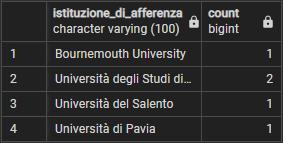
\includegraphics[width=6cm]{VIEW}
\caption{View in pgAdmin}
\end{figure}
\newpage
\subsection{Popolamento del database}
\begin{lstlisting}[language=SQL,
        deletekeywords={IDENTITY,INT},
        morekeywords={clustered},    
        framesep=10pt,
        framextopmargin=10pt]
--popolo la tabella SEDE:
INSERT INTO SEDE(NomeSede,NomeVia,NumeroCivico,Citta)
VALUES('convitto palmieri','piazzetta carducci',28,'lecce');

INSERT INTO SEDE(NomeSede,NomeVia,NumeroCivico,Citta)
VALUES('monte sant''angelo','via cintia',21,'napoli');

INSERT INTO SEDE(NomeSede,NomeVia,NumeroCivico,Citta)
VALUES('porta di massa', 'via porta di massa',1, 'napoli');





--popolo la tabella LOCAZIONE:
INSERT INTO LOCAZIONE (NomeLocazione, NomeSede)
VALUES('Athena','monte sant''angelo');

INSERT INTO LOCAZIONE (NomeLocazione, NomeSede)
VALUES('Nafsika','monte sant''angelo');

INSERT INTO LOCAZIONE (NomeLocazione, NomeSede)
VALUES('Sala d''arte (First floor)','convitto palmieri');

INSERT INTO LOCAZIONE (NomeLocazione, NomeSede)
VALUES('Sala Museo della Stampa','convitto palmieri');

INSERT INTO LOCAZIONE (NomeLocazione, NomeSede)
VALUES('Teatrino','convitto palmieri');

INSERT INTO LOCAZIONE (NomeLocazione, NomeSede)
VALUES('Sala sul Chiostro del 500 (First floor)','convitto palmieri');

INSERT INTO LOCAZIONE (NomeLocazione, NomeSede)
VALUES('Chiostro del 500','convitto palmieri');

INSERT INTO LOCAZIONE (NomeLocazione, NomeSede)
VALUES('AulaP','porta di massa');

INSERT INTO LOCAZIONE (NomeLocazione, NomeSede)
VALUES('Sala Grande','porta di massa');





--popolo la tabella CONFERENZA:
INSERT INTO CONFERENZA(TitoloConferenza,DataInizio,DataFine,Descrizione,NomeSede)
VALUES('21st International Conference on Image Analysis and Processing', '23/05/2022','27/05/2022',
	  'ICIAP: 21st International Conference on image analysis and processing 24 May 2022
	   Vi aspettiamo a ICIAP, la Conferenza organizzata ogni due anni dall''Association for
	   Research in Computer Vision, Pattern Recognition and Machine Learning (CVPL, ex
	   GIRPR) che e'' parte dell''International Association for Pattern Recognition (IAPR).','convitto palmieri');
	

   
INSERT INTO CONFERENZA(TitoloConferenza,DataInizio,DataFine,Descrizione,NomeSede)
VALUES('IEEE CSR CyberSecurity and Resilience', '27/07/2022','29/07/2022',
	  'The IEEE International Conference on Cyber Security and Resilience recognizes outstanding individuals
	   who make substantial contributions to the advancement of
	   security and resilience, inspiring other members of the community with their pioneering
	   research and innovation. The awardees need not be IEEE members.','monte sant''angelo');





--popolo la tabella SPONSOR:
INSERT INTO SPONSOR(PartitaIVA,NomeAzienda)
VALUES('04935230963','Apple Retail Italia S.r.l.');

INSERT INTO SPONSOR(PartitaIVA,NomeAzienda)
VALUES('11325690151','Samsung Electronics Italia S.p.A.');

INSERT INTO SPONSOR(PartitaIVA,NomeAzienda)
VALUES('00348270133','META S.P.A.');





--popolo la tabella PROGRAMMA:
INSERT INTO PROGRAMMA(DataProgramma,CodConferenza)
VALUES('23/05/2022',1);

INSERT INTO PROGRAMMA(DataProgramma,CodConferenza)
VALUES('24/05/2022',1);

INSERT INTO PROGRAMMA(DataProgramma,CodConferenza)
VALUES('25/05/2022',1);

INSERT INTO PROGRAMMA(DataProgramma,CodConferenza)
VALUES('26/05/2022',1);

INSERT INTO PROGRAMMA(DataProgramma,CodConferenza)
VALUES('27/05/2022',1);

INSERT INTO PROGRAMMA(DataProgramma,CodConferenza)
VALUES('27/07/2022',2);

INSERT INTO PROGRAMMA(DataProgramma,CodConferenza)
VALUES('28/07/2022',2);

INSERT INTO PROGRAMMA(DataProgramma,CodConferenza)
VALUES('29/07/2022',2);





--popolo la tabella INTERVALLO:
INSERT INTO INTERVALLO(TipoIntervallo,OrarioInizioIntervallo,OrarioFineIntervallo,CodProgramma)
VALUES('CoffeBreak', '10:30:00','11:00:00',0);

INSERT INTO INTERVALLO(TipoIntervallo,OrarioInizioIntervallo,OrarioFineIntervallo,CodProgramma)
VALUES('CoffeBreak','15:30:00','16:00:00',0);

INSERT INTO INTERVALLO(TipoIntervallo,OrarioInizioIntervallo,OrarioFineIntervallo,CodProgramma)
VALUES('CoffeBreak','10:30:00','11:00:00',1);

INSERT INTO INTERVALLO(TipoIntervallo,OrarioInizioIntervallo,OrarioFineIntervallo,CodProgramma)
VALUES('Pranzo','13:00:00','14:00:00',1);

INSERT INTO INTERVALLO(TipoIntervallo,OrarioInizioIntervallo,OrarioFineIntervallo,CodProgramma)
VALUES('CoffeBreak','15:30:00','16:00:00',1);

INSERT INTO INTERVALLO(TipoIntervallo,OrarioInizioIntervallo,OrarioFineIntervallo,CodProgramma)
VALUES('CoffeBreak','10:30:00','11:00:00',2);

INSERT INTO INTERVALLO(TipoIntervallo,OrarioInizioIntervallo,OrarioFineIntervallo,CodProgramma)
VALUES('Pranzo','13:00:00','14:00:00',2);

INSERT INTO INTERVALLO(TipoIntervallo,OrarioInizioIntervallo,OrarioFineIntervallo,CodProgramma)
VALUES('CoffeBreak','10:30:00','11:00:00',3);

INSERT INTO INTERVALLO(TipoIntervallo,OrarioInizioIntervallo,OrarioFineIntervallo,CodProgramma)
VALUES('Pranzo','13:00:00','14:00:00',3);

INSERT INTO INTERVALLO(TipoIntervallo,OrarioInizioIntervallo,OrarioFineIntervallo,CodProgramma)
VALUES('CoffeBreak','15:30:00','16:00:00',3);

INSERT INTO INTERVALLO(TipoIntervallo,OrarioInizioIntervallo,OrarioFineIntervallo,CodProgramma)
VALUES('CoffeBreak','10:30:00','11:00:00',4);

INSERT INTO INTERVALLO(TipoIntervallo,OrarioInizioIntervallo,OrarioFineIntervallo,CodProgramma)
VALUES('Pranzo','13:00:00','14:00:00',4);

INSERT INTO INTERVALLO(TipoIntervallo,OrarioInizioIntervallo,OrarioFineIntervallo,CodProgramma)
VALUES('CoffeBreak','15:30:00','16:00:00',4);

INSERT INTO INTERVALLO(TipoIntervallo,OrarioInizioIntervallo,OrarioFineIntervallo,CodProgramma)
VALUES('CoffeBreak','11:40:00','12:00:00',5);

INSERT INTO INTERVALLO(TipoIntervallo,OrarioInizioIntervallo,OrarioFineIntervallo,CodProgramma)
VALUES('Pranzo','13:20:00','14:20:00',5);

INSERT INTO INTERVALLO(TipoIntervallo,OrarioInizioIntervallo,OrarioFineIntervallo,CodProgramma)
VALUES('CoffeBreak','16:00:00','16:20:00',5);

INSERT INTO INTERVALLO(TipoIntervallo,OrarioInizioIntervallo,OrarioFineIntervallo,CodProgramma)
VALUES('CoffeBreak','11:40:00','12:00:00',6);

INSERT INTO INTERVALLO(TipoIntervallo,OrarioInizioIntervallo,OrarioFineIntervallo,CodProgramma)
VALUES('Pranzo','13:20:00','14:20:00',6);

INSERT INTO INTERVALLO(TipoIntervallo,OrarioInizioIntervallo,OrarioFineIntervallo,CodProgramma)
VALUES('CoffeBreak','18:00:00','18:20:00',6);

INSERT INTO INTERVALLO(TipoIntervallo,OrarioInizioIntervallo,OrarioFineIntervallo,CodProgramma)
VALUES('CoffeBreak','11:40:00','12:00:00',7);

INSERT INTO INTERVALLO(TipoIntervallo,OrarioInizioIntervallo,OrarioFineIntervallo,CodProgramma)
VALUES('Pranzo','13:20:00','14:20:00',7);





--popolo la tabella EVENTO_SOCIALE:
INSERT INTO EVENTO_SOCIALE(TipoEvento,OrarioInizioEvento,OrarioFineEvento,CodProgramma)
VALUES('Cena','19:30:00','22:00:00',2);

INSERT INTO EVENTO_SOCIALE(TipoEvento,OrarioInizioEvento,OrarioFineEvento,CodProgramma)
VALUES('Cena','18:50:00','23:30:00',3);

INSERT INTO EVENTO_SOCIALE(TipoEvento,OrarioInizioEvento,OrarioFineEvento,CodProgramma)
VALUES('Gita','18:50:00','23:30:00',4);





--popolo la tabella ENTE:
INSERT INTO ENTE(NomeIstituzione)
VALUES('Universita degli Studi di Napoli Federico II');

INSERT INTO ENTE(NomeIstituzione)
VALUES('Universita Parthenope');

INSERT INTO ENTE(NomeIstituzione)
VALUES('Universita del Salento');

INSERT INTO ENTE(NomeIstituzione)
VALUES('Universita Vanvitelli');

INSERT INTO ENTE(NomeIstituzione)
VALUES('Universita degli Studi di Salerno');

INSERT INTO ENTE(NomeIstituzione)
VALUES('University of Cambridge');

INSERT INTO ENTE(NomeIstituzione)
VALUES('Universita di Pavia');

INSERT INTO ENTE(NomeIstituzione)
VALUES('Bournemouth University');

INSERT INTO ENTE(NomeIstituzione)
VALUES('Humanitas University');

INSERT INTO ENTE(NomeIstituzione)
VALUES('University of Zilina');

INSERT INTO ENTE(NomeIstituzione)
VALUES('University of Alicante');

INSERT INTO ENTE(NomeIstituzione)
VALUES('Universita di Catania');





--popolo la tabella ORGANIZZATORE_LOCALE:
INSERT INTO ORGANIZZATORE_LOCALE(emailL,password,Titolo,Nome,Cognome,Istituzione_di_Afferenza)
VALUES('CarmenBisogni@unisa.it','Conferenze1000','Mss', 'Carmen','Bisogni', 'Universita degli Studi di Salerno');

INSERT INTO ORGANIZZATORE_LOCALE(emailL,password,Titolo,Nome,Cognome,Istituzione_di_Afferenza)
VALUES('PiercarloDondi@unipa.it','Conferenze1000','Professor', 'Piercarlo','Dondi', 'Universita di Pavia');

INSERT INTO ORGANIZZATORE_LOCALE(emailL,password,Titolo,Nome,Cognome,Istituzione_di_Afferenza)
VALUES('FabioNarducci@unisa.it','Conferenze1000','Mr', 'Fabio','Narducci', 'Universita degli Studi di Salerno');

INSERT INTO ORGANIZZATORE_LOCALE(emailL,password,Titolo,Nome,Cognome,Istituzione_di_Afferenza)
VALUES('AlessandroBruno@gmail.it','Conferenze1000','Mr', 'Alessandro','Bruno', 'Humanitas University');

INSERT INTO ORGANIZZATORE_LOCALE(emailL,password,Titolo,Nome,Cognome,Istituzione_di_Afferenza)
VALUES('SimonePalazzo@unica.it','Conferenze1000','Mr', 'Simone','Palazzo', 'Universita di Catania');

INSERT INTO ORGANIZZATORE_LOCALE(emailL,password,Titolo,Nome,Cognome,Istituzione_di_Afferenza)
VALUES('FedericaProiettoSalanitri@unisa.it','Conferenze1000','Mss', 'Federica','Proietto Salanitri', 'Universita di Catania');

INSERT INTO ORGANIZZATORE_LOCALE(emailL,password,Titolo,Nome,Cognome,Istituzione_di_Afferenza)
VALUES('VincenzoLomonaco@unipa.it','Conferenze1000','Professor', 'Vincenzo','Lomonaco', 'Universita di Pavia');






--popolo la tabella ORGANIZZATORE_SCIENTIFICO:
INSERT INTO ORGANIZZATORE_SCIENTIFICO(emailS,password,Titolo,Nome,Cognome,
Istituzione_di_Afferenza)
VALUES('ZoheirSabeur@gmail.com','Conferenze1000','Professor','Zoheir','Sabeur',
'Bournemouth University');



INSERT INTO ORGANIZZATORE_SCIENTIFICO(emailS,password,Titolo,Nome,Cognome,
Istituzione_di_Afferenza)
VALUES('DenizChetinkaya@gmail.com','Conferenze1000','Professoressa', 'Deniz','Chetinkaya', 'Bournemouth University');

INSERT INTO ORGANIZZATORE_SCIENTIFICO(emailS,password,Titolo,Nome,Cognome,
Istituzione_di_Afferenza)
VALUES('FranciscoFlorez-Revuelta@gmail.com','Conferenze1000','Mr', 'Francisco','Florez-Revuelta', 'University of Alicante');

INSERT INTO ORGANIZZATORE_SCIENTIFICO(emailS,password,Titolo,Nome,Cognome,
Istituzione_di_Afferenza)
VALUES('PeterPocta@gmail.com','Conferenze1000','Mr', 'Peter','Pocta', 'University of Zilina');

INSERT INTO ORGANIZZATORE_SCIENTIFICO(emailS,password,Titolo,Nome,Cognome,
Istituzione_di_Afferenza)
VALUES('JonAnderGomezAdrian@gmail.com','Conferenze1000','Mr', 'Jon Ander','Gomez Adrian', 'University of Alicante');

INSERT INTO ORGANIZZATORE_SCIENTIFICO(emailS,password,Titolo,Nome,Cognome,
Istituzione_di_Afferenza)
VALUES('StephenHawking@gmail.com','Conferenze1000','Mr', 'Stephen','Hawking', 'University of Cambridge');






--popolo la tabella PARTECIPANTE:
INSERT INTO PARTECIPANTE(emailP, Titolo, Nome, Cognome, Istituzione_di_Afferenza)
VALUES('NicolaLerme@unipa.it','Mr','Nicola','Lerme','Universita di Pavia');

INSERT INTO PARTECIPANTE(emailP, Titolo, Nome, Cognome, Istituzione_di_Afferenza)
VALUES('LorenzoBaraldi@unina.it','Mr','Lorenzo', 'Baraldi', 'Universita degli Studi di Napoli Federico II');

INSERT INTO PARTECIPANTE(emailP, Titolo, Nome, Cognome, Istituzione_di_Afferenza)
VALUES('AlessandroGrieco@unina.it','Mr','Alessandro','Grieco','Universita degli Studi di Napoli Federico II');

INSERT INTO PARTECIPANTE(emailP, Titolo, Nome, Cognome, Istituzione_di_Afferenza)
VALUES('StefanoAllegretti@unipart.it','Mr','Stefano','Allegretti','Universita Parthenope');

INSERT INTO PARTECIPANTE(emailP, Titolo, Nome, Cognome, Istituzione_di_Afferenza)
VALUES('DarioMoccia@unipart.it','Professor','Dario', 'Moccia','Universita Parthenope');

INSERT INTO PARTECIPANTE(emailP, Titolo, Nome, Cognome, Istituzione_di_Afferenza)
VALUES('ClaudioFerrari@unica.it','Professor','Claudio','Ferrari','Universita di Catania');

INSERT INTO PARTECIPANTE(emailP, Titolo, Nome, Cognome, Istituzione_di_Afferenza)
VALUES('FedericoBeccaria@univa.it','Mr','Federico','Beccaria','Universita Vanvitelli');

INSERT INTO PARTECIPANTE(emailP, Titolo, Nome, Cognome, Istituzione_di_Afferenza)
VALUES('AndreaPilzer@univa.it','Professor','Andrea','Pizler','Universita Vanvitelli');

INSERT INTO PARTECIPANTE(emailP, Titolo, Nome, Cognome, Istituzione_di_Afferenza)
VALUES('GiovanniRana@gmail.com','Professor','Giovanni','Rana','Bournemouth University');

INSERT INTO PARTECIPANTE(emailP, Titolo, Nome, Cognome, Istituzione_di_Afferenza)
VALUES('CosimoDistante@unisal.it','Professor','Cosimo','Distante','Universita del Salento');

INSERT INTO PARTECIPANTE(emailP, Titolo, Nome, Cognome, Istituzione_di_Afferenza)
VALUES('FrancescoBarecchia@unina.it','Mr','Francesco','Barecchia','Universita degli Studi di Napoli Federico II');





--popolo la tabella ponte ORGANIZZARE_S:
INSERT INTO ORGANIZZARE_S(CodConferenza,emailS)
VALUES(1,'FranciscoFlorez-Revuelta@gmail.com');

INSERT INTO ORGANIZZARE_S(CodConferenza,emailS)
VALUES(1,'DenizChetinkaya@gmail.com');

INSERT INTO ORGANIZZARE_S(CodConferenza,emailS)
VALUES(1,'JonAnderGomezAdrian@gmail.com');

INSERT INTO ORGANIZZARE_S(CodConferenza,emailS)
VALUES(1,'PeterPocta@gmail.com');

INSERT INTO ORGANIZZARE_S(CodConferenza,emailS)
VALUES(1,'ZoheirSabeur@gmail.com');

INSERT INTO ORGANIZZARE_S(CodConferenza,emailS)
VALUES(1,'StephenHawking@gmail.com');

INSERT INTO ORGANIZZARE_S(CodConferenza,emailS)
VALUES(2,'FranciscoFlorez-Revuelta@gmail.com');

INSERT INTO ORGANIZZARE_S(CodConferenza,emailS)
VALUES(2,'DenizChetinkaya@gmail.com');





--popolo la tabella SESSIONE:
INSERT INTO SESSIONE(OrarioInizioSessione,OrarioFineSessione,TitoloSessione,DescrizioneSessione
,Chair,KeynoteSpeaker,CodProgramma,NomeLocazione)
VALUES('9:00:00','10:30:00','Parts can worth like the whole','Quite often the useful data for an analysis task are not available in an optimal condition. This may be due to the occlusions or the noise affecting the 
acquisition of the samples, or in some cases the problem itself is conceived in a way that a solution comes from the analysis of smaller portions of the input.', 
'FranciscoFlorez-Revuelta@gmail.com','NicolaLerme@unipa.it',0,'Sala sul Chiostro del 500 (First floor)');
	   
INSERT INTO SESSIONE(OrarioInizioSessione,OrarioFineSessione,TitoloSessione,DescrizioneSessione,
Chair,KeynoteSpeaker,CodProgramma,NomeLocazione)
VALUES('11:00','15:30','HBAxSCES - Human Behaviour Analysis for Smart City Environment Safety','Nowadays, Smart Cities aim to ensure secure and safe physical and digital environments for the well-being of citizens.
Among many, ICT systems are reliant on evolving Artificial Intelligence, Pattern Recognition, Computer Vision, 3D simulations and Digital Twins techniques to make the environments more resilient.',
'JonAnderGomezAdrian@gmail.com','GiovanniRana@gmail.com',0,'Teatrino');

INSERT INTO SESSIONE(OrarioInizioSessione,OrarioFineSessione,TitoloSessione,DescrizioneSessione,
Chair,CodProgramma,NomeLocazione)
VALUES('16:00','18:00','Deep Learning High Performance Computing to Boost Biomedical Applications','Healthcare is one of the key sectors of the global economy, especially in Europe. Any improvement in healthcare 
systems has a high impact on the welfare of the society. The use of technologies in health is clearly a strong path to more efficient healthcare, benefitting both individual people and the publicbudgets. European 
public health systems are generating large datasets of biomedical data in general, and images in particular, as most medical examinations use image-based processes.', 
'PeterPocta@gmail.com',0,'Sala d''arte (First floor)');

INSERT INTO SESSIONE(OrarioInizioSessione,OrarioFineSessione,TitoloSessione,DescrizioneSessione,
Chair,KeynoteSpeaker,CodProgramma,NomeLocazione)
VALUES('9:00','10:30','Deep Learning for Visual Object Tracking Pt1','In its simplest definition, visual object tracking consists in the persistent recognition and localization of a generic target object in a video. 
Several challenges such as object occlusions, pose and scale changes, rotations and shape variations, and the presence of similar objects, must be tackled to accurately keep track of a target''s position. The ultimate
goal of generic object tracking is to build robust models capable to overcome such challenging factors. In the past, such issues have been addressed by disparate principles formalizing the concepts of appearance
model, motion model, and matching operation. In recent years, algorithms based on deep learning tried to learn such conceptual blocks by exploiting the ability of deep neural networks in learning complex functions 
from visual examples.','ZoheirSabeur@gmail.com','AlessandroGrieco@unina.it',1,'Teatrino');
	   
INSERT INTO SESSIONE(OrarioInizioSessione,OrarioFineSessione,TitoloSessione,DescrizioneSessione,
Chair,KeynoteSpeaker,CodProgramma,NomeLocazione)
VALUES('11:00','13:00','Deep Learning for Visual Object Tracking Pt2','In its simplest definition, visual object tracking consists in the persistent recognition and localization of a generic target object in a video.
Several challenges such as object occlusions, pose and scale changes, rotations and shape variations, and the presence of similar objects, must be tackled to accurately keep track of a target''s position. The ultimate
goal of generic object tracking is to build robust models capable to overcome such challenging factors. In the past, such issues have been addressed by disparate principles formalizing the concepts of appearance model,
motion model, and matching operation. In recent years, algorithms based on deep learning tried to learn such conceptual blocks by exploiting the ability of deep neural networks in learning complex functions from visual 
examples.','ZoheirSabeur@gmail.com','AlessandroGrieco@unina.it',1,'Teatrino');	   

INSERT INTO SESSIONE(OrarioInizioSessione,OrarioFineSessione,TitoloSessione,DescrizioneSessione,
Chair,CodProgramma,NomeLocazione)
VALUES('11:00','13:00',' WOSDETC - Small-Drone Surveillance, Detection and Counteraction Techniques','In the last few years the popularity of small Remotely Piloted Aircraft Systems (RPAS) and more generally (also 
autonomous) "drones", has exponentially increased due to the availability of low-cost off-the-shelf products, including build-from-scratch and DIY kits. At the same time, issues regarding safety, privacy and security 
aspects are arising. There is inded a gap in current surveillance systems for the detection of such flying systems, which can be used for illegal activities such as smuggling of drugs or espionage, as well as for
carrying explosives or chemical weapons.','PeterPocta@gmail.com',1,'Sala sul Chiostro del 500 (First floor)');

INSERT INTO SESSIONE(OrarioInizioSessione,OrarioFineSessione,TitoloSessione,DescrizioneSessione,
Chair,KeynoteSpeaker,CodProgramma,NomeLocazione)
VALUES('14:00','15:30','DEEP LEARNING FOR MULTI-GPUS','Deep Learning has been the most significant breakthrough in the past 10 years in the field of pattern recognition and machine learning. It has achieved significant
advancements in terms of the effectiveness of prediction models on many research topics and application fields, ranging from computer vision, natural language processing, embodied AI and to more traditional fields of 
pattern recognition. This paradigm shift has radically changed the research methodology towards a data-oriented approach, in which learning involves all steps of the prediction pipeline from feature extraction to
classification.','JonAnderGomezAdrian@gmail.com','FrancescoBarecchia@unina.it',1,
'Teatrino');
	   
INSERT INTO SESSIONE(OrarioInizioSessione,OrarioFineSessione,TitoloSessione,
Chair,CodProgramma,NomeLocazione)
VALUES('8:30','10:30','Oral Session 1: Image Analysis, Detection and Recognition','ZoheirSabeur@gmail.com',2,'Sala d''arte (First floor)');

INSERT INTO SESSIONE(OrarioInizioSessione,OrarioFineSessione,TitoloSessione,
Chair,CodProgramma,NomeLocazione)
VALUES('14:00','15:30','Message from the General Chair','DenizChetinkaya@gmail.com',2,'Teatrino');

INSERT INTO SESSIONE(OrarioInizioSessione,OrarioFineSessione,TitoloSessione,DescrizioneSessione,
Chair,KeynoteSpeaker,CodProgramma,NomeLocazione)
VALUES('11:00','13:00','Industrial Panel','The Industrial Panel session will start with presentations by the panelists, introducing the companies and the technological challenges of their business.',
		'PeterPocta@gmail.com','CosimoDistante@unisal.it',3,'Sala Museo della Stampa');

INSERT INTO SESSIONE(OrarioInizioSessione,OrarioFineSessione,TitoloSessione,
Chair,CodProgramma,NomeLocazione)
VALUES('14:00','15:30','Shifting paradigms in multi-object tracking','FranciscoFlorez-Revuelta@gmail.com',3,'Sala Museo della Stampa');

INSERT INTO SESSIONE(OrarioInizioSessione,OrarioFineSessione,TitoloSessione,DescrizioneSessione,
Chair,KeynoteSpeaker,CodProgramma,NomeLocazione)
VALUES('11:00','13:00','Video Understanding - An Egocentric Perspective','This talk aims to argue for a fine(r)-grained perspective onto human-object interactions, from video sequences, captured 
 in an egocentric perspective (i.e. first-person footage).', 'FranciscoFlorez-Revuelta@gmail.com','NicolaLerme@unipa.it',4,'Sala d''arte (First floor)');

INSERT INTO SESSIONE(OrarioInizioSessione,OrarioFineSessione,TitoloSessione,
Chair,CodProgramma,NomeLocazione)
VALUES('14:00','15:30','Closing remarks','StephenHawking@gmail.com',4,'Sala Museo della Stampa');

INSERT INTO SESSIONE(OrarioInizioSessione,OrarioFineSessione,TitoloSessione,
Chair,CodProgramma,NomeLocazione)
VALUES('9:00','10:00','Plenary session PL-1','FranciscoFlorez-Revuelta@gmail.com',5,'Athena');

INSERT INTO SESSIONE(OrarioInizioSessione,OrarioFineSessione,TitoloSessione,
Chair,CodProgramma,NomeLocazione)
VALUES('10:00','11:40','CSR-1','FranciscoFlorez-Revuelta@gmail.com',5,'Athena');

INSERT INTO SESSIONE(OrarioInizioSessione,OrarioFineSessione,TitoloSessione,
Chair,CodProgramma,NomeLocazione)
VALUES('12:00','13:20','CSR-2','FranciscoFlorez-Revuelta@gmail.com',5,'Athena');

INSERT INTO SESSIONE(OrarioInizioSessione,OrarioFineSessione,TitoloSessione,
Chair,CodProgramma,NomeLocazione)
VALUES('14:20','16:00','CSR-3','FranciscoFlorez-Revuelta@gmail.com',5,'Athena');

INSERT INTO SESSIONE(OrarioInizioSessione,OrarioFineSessione,TitoloSessione,
Chair,CodProgramma,NomeLocazione)
VALUES('16:20','18:00','CSR-2','FranciscoFlorez-Revuelta@gmail.com',5,'Athena');

INSERT INTO SESSIONE(OrarioInizioSessione,OrarioFineSessione,TitoloSessione,
Chair,CodProgramma,NomeLocazione)
VALUES('10:00','11:40','WS-DS4CS-1','DenizChetinkaya@gmail.com',5,'Nafsika');

INSERT INTO SESSIONE(OrarioInizioSessione,OrarioFineSessione,TitoloSessione,
Chair,CodProgramma,NomeLocazione)
VALUES('12:00','13:20','CSR-2','DenizChetinkaya@gmail.com',5,'Nafsika');

INSERT INTO SESSIONE(OrarioInizioSessione,OrarioFineSessione,TitoloSessione,
Chair,CodProgramma,NomeLocazione)
VALUES('15:00','16:00','CSR-3','DenizChetinkaya@gmail.com',5,'Nafsika');

INSERT INTO SESSIONE(OrarioInizioSessione,OrarioFineSessione,TitoloSessione,
Chair,CodProgramma,NomeLocazione)
VALUES('16:20','18:00','CSR-2','DenizChetinkaya@gmail.com',5,'Nafsika');

INSERT INTO SESSIONE(OrarioInizioSessione,OrarioFineSessione,TitoloSessione,
Chair,CodProgramma,NomeLocazione)
VALUES('9:00','10:00','PL-2','FranciscoFlorez-Revuelta@gmail.com',6,'Athena');

INSERT INTO SESSIONE(OrarioInizioSessione,OrarioFineSessione,TitoloSessione,
Chair,CodProgramma,NomeLocazione)
VALUES('10:00','11:40','CSR-5','FranciscoFlorez-Revuelta@gmail.com',6,'Athena');

INSERT INTO SESSIONE(OrarioInizioSessione,OrarioFineSessione,TitoloSessione,
Chair,CodProgramma,NomeLocazione)
VALUES('12:00','13:20','CSR-6','FranciscoFlorez-Revuelta@gmail.com',6,'Athena');

INSERT INTO SESSIONE(OrarioInizioSessione,OrarioFineSessione,TitoloSessione,
Chair,CodProgramma,NomeLocazione)
VALUES('14:20','15:20','PL-3','FranciscoFlorez-Revuelta@gmail.com',6,'Athena');

INSERT INTO SESSIONE(OrarioInizioSessione,OrarioFineSessione,TitoloSessione,
Chair,CodProgramma,NomeLocazione)
VALUES('15:20','16:20','AW','FranciscoFlorez-Revuelta@gmail.com',6,'Athena');

INSERT INTO SESSIONE(OrarioInizioSessione,OrarioFineSessione,TitoloSessione,
Chair,CodProgramma,NomeLocazione)
VALUES('10:00','11:40','WS-CRE-1','DenizChetinkaya@gmail.com',6,'Nafsika');

INSERT INTO SESSIONE(OrarioInizioSessione,OrarioFineSessione,TitoloSessione,
Chair,CodProgramma,NomeLocazione)
VALUES('12:00','13:20','WS-CRST','DenizChetinkaya@gmail.com',6,'Nafsika');

INSERT INTO SESSIONE(OrarioInizioSessione,OrarioFineSessione,TitoloSessione,
Chair,CodProgramma,NomeLocazione)
VALUES('16:20','18:00','WS-CRE-2','DenizChetinkaya@gmail.com',6,'Nafsika');

INSERT INTO SESSIONE(OrarioInizioSessione,OrarioFineSessione,TitoloSessione,
Chair,CodProgramma,NomeLocazione)
VALUES('18:40','20:00','WS-CRE-3','DenizChetinkaya@gmail.com',6,'Nafsika');

INSERT INTO SESSIONE(OrarioInizioSessione,OrarioFineSessione,TitoloSessione,
Chair,CodProgramma,NomeLocazione)
VALUES('9:00','10:00','PL-4','FranciscoFlorez-Revuelta@gmail.com',7,'Athena');

INSERT INTO SESSIONE(OrarioInizioSessione,OrarioFineSessione,TitoloSessione,
Chair,CodProgramma,NomeLocazione)
VALUES('10:00','11:40','CSR-7','FranciscoFlorez-Revuelta@gmail.com',7,'Athena');

INSERT INTO SESSIONE(OrarioInizioSessione,OrarioFineSessione,TitoloSessione,
Chair,CodProgramma,NomeLocazione)
VALUES('12:00','13:20','CSR-8','FranciscoFlorez-Revuelta@gmail.com',7,'Athena');

INSERT INTO SESSIONE(OrarioInizioSessione,OrarioFineSessione,TitoloSessione,
Chair,CodProgramma,NomeLocazione)
VALUES('14:20','16:00','CSR-9','FranciscoFlorez-Revuelta@gmail.com',7,'Athena');

INSERT INTO SESSIONE(OrarioInizioSessione,OrarioFineSessione,TitoloSessione,
Chair,CodProgramma,NomeLocazione)
VALUES('10:00','11:40','WS-EPES-SPR','DenizChetinkaya@gmail.com',7,'Nafsika');

INSERT INTO SESSIONE(OrarioInizioSessione,OrarioFineSessione,TitoloSessione,
Chair,CodProgramma,NomeLocazione)
VALUES('14:20','16:00','WS-ACTI','DenizChetinkaya@gmail.com',7,'Nafsika');






--popolo la tabella INTERVENTO:
INSERT INTO INTERVENTO(codPartecipante,OrarioInizioIntervento,OrarioFineIntervento,CodSessione)
VALUES('AlessandroGrieco@unina.it','9:30','10:00',3);

INSERT INTO INTERVENTO(codPartecipante,OrarioInizioIntervento,OrarioFineIntervento,CodSessione)
VALUES('LorenzoBaraldi@unina.it','15:00','16:00',16);

INSERT INTO INTERVENTO(codPartecipante,OrarioInizioIntervento,OrarioFineIntervento,CodSessione)
VALUES('CosimoDistante@unisal.it','15:00','15:30',20);

INSERT INTO INTERVENTO(codPartecipante,OrarioInizioIntervento,OrarioFineIntervento,CodSessione)
VALUES('FrancescoBarecchia@unina.it','10:00','10:20',23);

INSERT INTO INTERVENTO(codPartecipante,OrarioInizioIntervento,OrarioFineIntervento,CodSessione)
VALUES('AlessandroGrieco@unina.it','10:20','10:40',23);

INSERT INTO INTERVENTO(codPartecipante,OrarioInizioIntervento,OrarioFineIntervento,CodSessione)
VALUES('ClaudioFerrari@unica.it','13:00','13:20',15);





--popolo la tabella ponte ORGANIZZARE_L:
INSERT INTO ORGANIZZARE_L(CodConferenza,emailL)
VALUES(1,'CarmenBisogni@unisa.it');

INSERT INTO ORGANIZZARE_L(CodConferenza,emailL)
VALUES(1,'FabioNarducci@unisa.it');

INSERT INTO ORGANIZZARE_L(CodConferenza,emailL)
VALUES(1,'FedericaProiettoSalanitri@unisa.it');

INSERT INTO ORGANIZZARE_L(CodConferenza,emailL)
VALUES(1,'SimonePalazzo@unica.it');

INSERT INTO ORGANIZZARE_L(CodConferenza,emailL)
VALUES(2,'CarmenBisogni@unisa.it');

INSERT INTO ORGANIZZARE_L(CodConferenza,emailL)
VALUES(2,'FabioNarducci@unisa.it');

INSERT INTO ORGANIZZARE_L(CodConferenza,emailL)
VALUES(2,'AlessandroBruno@gmail.it');

INSERT INTO ORGANIZZARE_L(CodConferenza,emailL)
VALUES(2,'PiercarloDondi@unipa.it');

INSERT INTO ORGANIZZARE_L(CodConferenza,emailL)
VALUES(2,'VincenzoLomonaco@unipa.it');





--popolo la tabella ponte PARTECIPARE:
INSERT INTO PARTECIPARE(CodSessione,emailP)
VALUES(15,'NicolaLerme@unipa.it');

INSERT INTO PARTECIPARE(CodSessione,emailP)
VALUES(15,'ClaudioFerrari@unica.it');

INSERT INTO PARTECIPARE(CodSessione,emailP)
VALUES(16,'ClaudioFerrari@unica.it');

INSERT INTO PARTECIPARE(CodSessione,emailP)
VALUES(16,'LorenzoBaraldi@unina.it');

INSERT INTO PARTECIPARE(CodSessione,emailP)
VALUES(11,'ClaudioFerrari@unica.it');

INSERT INTO PARTECIPARE(CodSessione,emailP)
VALUES(13,'LorenzoBaraldi@unina.it');

INSERT INTO PARTECIPARE(CodSessione,emailP)
VALUES(4,'GiovanniRana@gmail.com');

INSERT INTO PARTECIPARE(CodSessione,emailP)
VALUES(7,'GiovanniRana@gmail.com');

INSERT INTO PARTECIPARE(CodSessione,emailP)
VALUES(5,'CosimoDistante@unisal.it');

INSERT INTO PARTECIPARE(CodSessione,emailP)
VALUES(20,'CosimoDistante@unisal.it');

INSERT INTO PARTECIPARE(CodSessione,emailP)
VALUES(23,'FrancescoBarecchia@unina.it');

INSERT INTO PARTECIPARE(CodSessione,emailP)
VALUES(23,'AlessandroGrieco@unina.it');





--popolo la tabella ponte PUBBLICITA':
INSERT INTO pubblicita(PartitaIVA, CodConferenza, Spesa)
VALUES('00348270133', 2, 200000);

INSERT INTO pubblicita(PartitaIVA, CodConferenza, Spesa)
VALUES('04935230963', 1, 150000);

INSERT INTO pubblicita(PartitaIVA, CodConferenza, Spesa)
VALUES('11325690151', 1, 75000);
\end{lstlisting}

\end{document}
